% Created 2020-06-20 Sat 12:34
% Intended LaTeX compiler: pdflatex
\documentclass[11pt]{article}
\usepackage[utf8]{inputenc}
\usepackage[T1]{fontenc}
\usepackage{graphicx}
\usepackage{grffile}
\usepackage{longtable}
\usepackage{wrapfig}
\usepackage{rotating}
\usepackage[normalem]{ulem}
\usepackage{amsmath}
\usepackage{textcomp}
\usepackage{amssymb}
\usepackage{capt-of}
\usepackage{hyperref}
\usepackage{minted}
\author{Dustin Leatherman}
\date{\today}
\title{Class Notes}
\hypersetup{
 pdfauthor={Dustin Leatherman},
 pdftitle={Class Notes},
 pdfkeywords={},
 pdfsubject={},
 pdfcreator={Emacs 26.3 (Org mode 9.4)}, 
 pdflang={English}}
\begin{document}

\maketitle
\tableofcontents


\section{Review \& Introduction (2020/03/31)}
\label{sec:orgffc0028}
\subsection{Review}
\label{sec:orgf6076de}
\textbf{Orthogonal}: Vectors are orthogonal when the dot product = 0.
\subsubsection{Basis}
\label{sec:org298e664}

\begin{equation}
\begin{split}
\underset{(n \times 1)}{\vec{y}} = & \underset{(n \times p)}{A} \underset{(p \times 1)}{\vec{x}}\\
= & B \vec{c} \\
= & \Sigma c_i \vec{b_i} \ \text{(most $c_i$ = 0)}
\end{split}
\end{equation}

\textbf{A}: Basis Matrix

\textbf{Properties of a Good Basis}
\begin{itemize}
\item not all are orthogonal
\item Allows for a sparse vector to be used ad the constant vector \(\vec{c}\)
\end{itemize}

Identity Matrices are the \emph{worst} basis because most coefficients are non-zero.

\textbf{2-Sparse Vector}
\begin{equation}
\begin{split}
\vec{c} = \begin{bmatrix}
0\\
0\\
0\\
0\\
3\\
0\\
0\\
4
\end{bmatrix}
\end{split}
\end{equation}


Very important!
\begin{quote}
When dealing with Natural images and a good basis, there is a sparse vector.
\end{quote}

\subsubsection{Kernel}
\label{sec:orgeb880ab}
The kernel of a linear mapping is the set of
vectors mapped to the 0 vector. The kernel is often referred to as the \textbf{null
space}. Vectors should be linearly independent.

\begin{equation}
\begin{split}
Ker(A) = { \vec{x} \in \mathbb{R}^n \colon A \vec{x} = \vec{0}}
\end{split}
\end{equation}

A must be designed such that the Kernel of A does not contain any s-sparse
vector other than \(\vec 0\)

\textbf{Main Idea}: For (1), reduce \(\vec{y}\) to a K-Sparse matrix to reduce the amount
of non-zero numbers.

\subsection{Linear Algebra Review}
\label{sec:org9882e5c}
\begin{equation}
\begin{split}
\vec{u} = \begin{bmatrix}
1\\
2\\
-1
\end{bmatrix},
\vec{v} = \begin{bmatrix}
1\\
1\\
2
\end{bmatrix}
\end{split}
\end{equation}

\begin{equation}
\begin{split}
\underset{(1 \times 3)(3 \times 1)}{\vec{u}^T \vec{v}} = & \begin{bmatrix}
1 & 2 & -1
\end{bmatrix}\begin{bmatrix}
1\\
1\\
2
\end{bmatrix} = 1 + 2 - 2 = 1\\
= & \vec{u} \cdot \vec{v}
\end{split}
\end{equation}

\begin{equation}
\begin{split}
\underset{(3 \times 1)(1 \times 3)}{\vec{u} \ \vec{v}^T} = \begin{bmatrix}
1\\
2\\
-1
\end{bmatrix}\begin{bmatrix}
1 & 1 & 2
\end{bmatrix} = \begin{bmatrix}
1 & 1 & 2\\
2 & 2 & 4\\
-1 & -1 & -2
\end{bmatrix}
\end{split}
\end{equation}

\(\vec{u} \ \vec{v}^T \neq \vec{u}^T \ \vec{v}\)

\subsubsection{Inner Product}
\label{sec:org41b1b99}

\begin{equation}
\begin{split}
<\vec{a}, \vec{b}> = & \vec{a} \cdot \vec{b}\\
= & \vec{a}^T \vec{b}
\end{split}
\end{equation}

\subsubsection{Cauchy-Schwartz Inequality}
\label{sec:orgb0b6da9}

\begin{equation}
\begin{split}
\vec{a} = \begin{bmatrix}
1\\
2\\
-1
\end{bmatrix}, \begin{bmatrix}
1\\
1\\
2
\end{bmatrix}
\end{split}
\end{equation}

\begin{equation}
\begin{split}
& |<\vec{a}, \vec{b}>| \leq \sqrt{1^2 + 2^2 + (-1)^2} \times \sqrt{1^2 + 1^2 + 2^2} \\
& |<\vec{a}, \vec{b}>| \leq ||\vec{a}||_2 \ ||\vec{b}||_2 \ \text{(euclidean/l2-norm)}
\end{split}
\end{equation}

\subsubsection{Norms}
\label{sec:org326028b}

Why is the l1 norm preferred for ML opposed to the classic l2 norm?

Philosophically,

If we looked at a sphere in l2 norm, the shadow casted would be a circle
regardless of the direction of the light.

Looking at a sphere in the l1 norm is shaped as a tetrahedron. The shadow cast
by a tetrahedron is different for different angles so observing the shadow
provides a lot more context about the sphere.

\begin{enumerate}
\item Euclidean/l2
\label{sec:orga249345}

\textbf{Sphere}: \(||\vec{x}||_2 = \sqrt{(-4)^2 + 3^2} = \sqrt{25} = 5\)

\begin{enumerate}
\item FOIL
\label{sec:org4fb89ae}
Given 2 fixed vectors x,y. Consider the l2-norm squared:

$$
f(t) = ||x + ty||_2^2
$$


\begin{equation}
\begin{split}
f(t) = & ||x + ty||_2^2\\
= & <x + ty, x+ ty>\\
= & <x,x> + t <x, y> + t <y, x> + t^2 <y, y>\\
= & ||x||_2^2 + 2t<x,y> + t^2 ||y||_2^2
\end{split}
\end{equation}

\begin{quote}
Note: t<x,y> and t<y,x> can be combined because their dot-products are
equivalent. \(\vec{x} \cdot \vec{y} = \vec{y} \cdot \vec{x}\)
\end{quote}

\begin{quote}
When using Machine Learning, don't use l2 norms. Use l1
\end{quote}

\item Derivative
\label{sec:orgb665491}

\begin{equation}
\begin{split}
\frac{d}{dt}(||x + ty||_2^2) = & 2<x, y> + 2t ||y||_2^2\\
= & 2 x^T y + 2t y^T y
\end{split}
\end{equation}
\end{enumerate}

\item Simplex/l1
\label{sec:org035a783}

\textbf{Sphere}: \(||\vec{x}||_1 = |-4| + |3| = 7\)

\item Infinity
\label{sec:org7defd09}

\textbf{Sphere}: \(||\vec{x}||_\infty = Max{|-4|, |3|} = 4\)
\end{enumerate}
\subsection{Optimization}
\label{sec:org5e91cad}

Why is Machine Learning Possible? Is there a theoretical guarantee?

\begin{center}
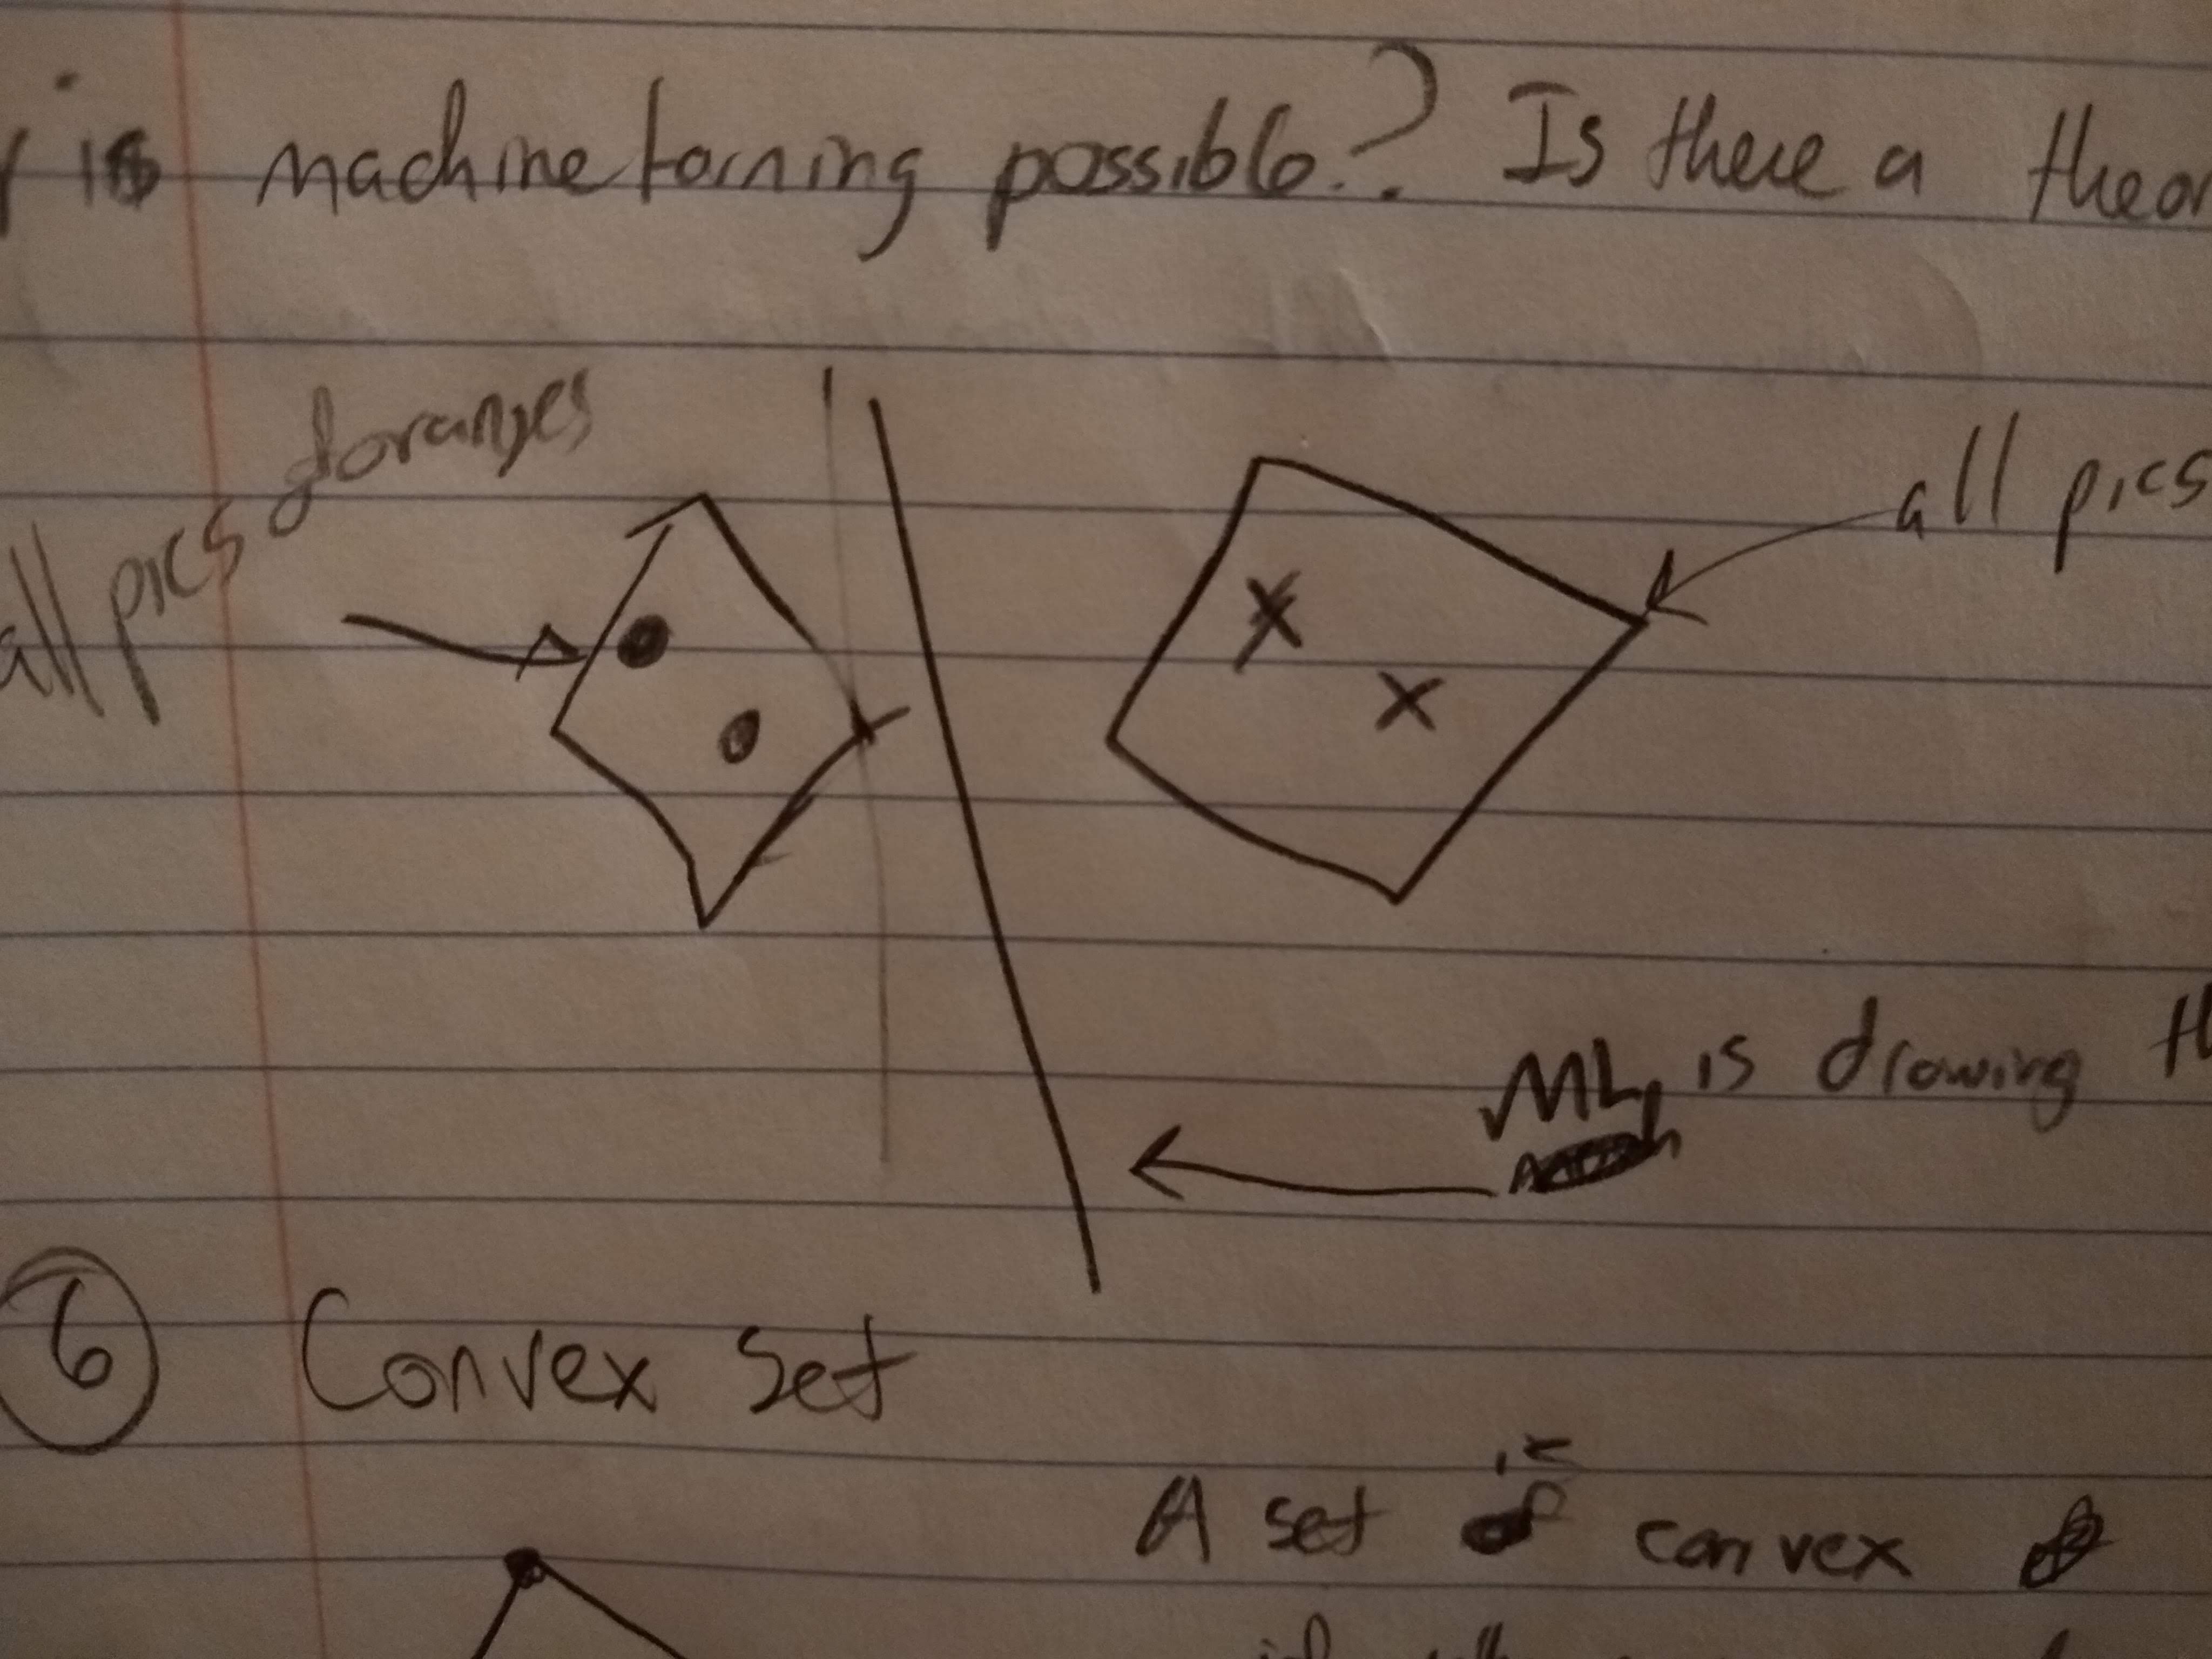
\includegraphics[width=.9\linewidth]{./resources/convex2.jpg}
\end{center}

Imagine A is the set of all dogs and B is the set of all Cats

If the sets are convex and do not overlap, there exists a line between them
which acts as a divider for determining whether a new pic belongs in A or B.

\subsection{Convex Set}
\label{sec:org2c8cab6}

A set is convex if whenever X and Y are in the set, then for \(0 \leq t \leq 1\)
the points \((1 - t)x + ty\) must also be in the set.

\begin{itemize}
\item \#+ATTR\textsubscript{\LaTeX{}}: scale=0.5
\end{itemize}
\begin{center}
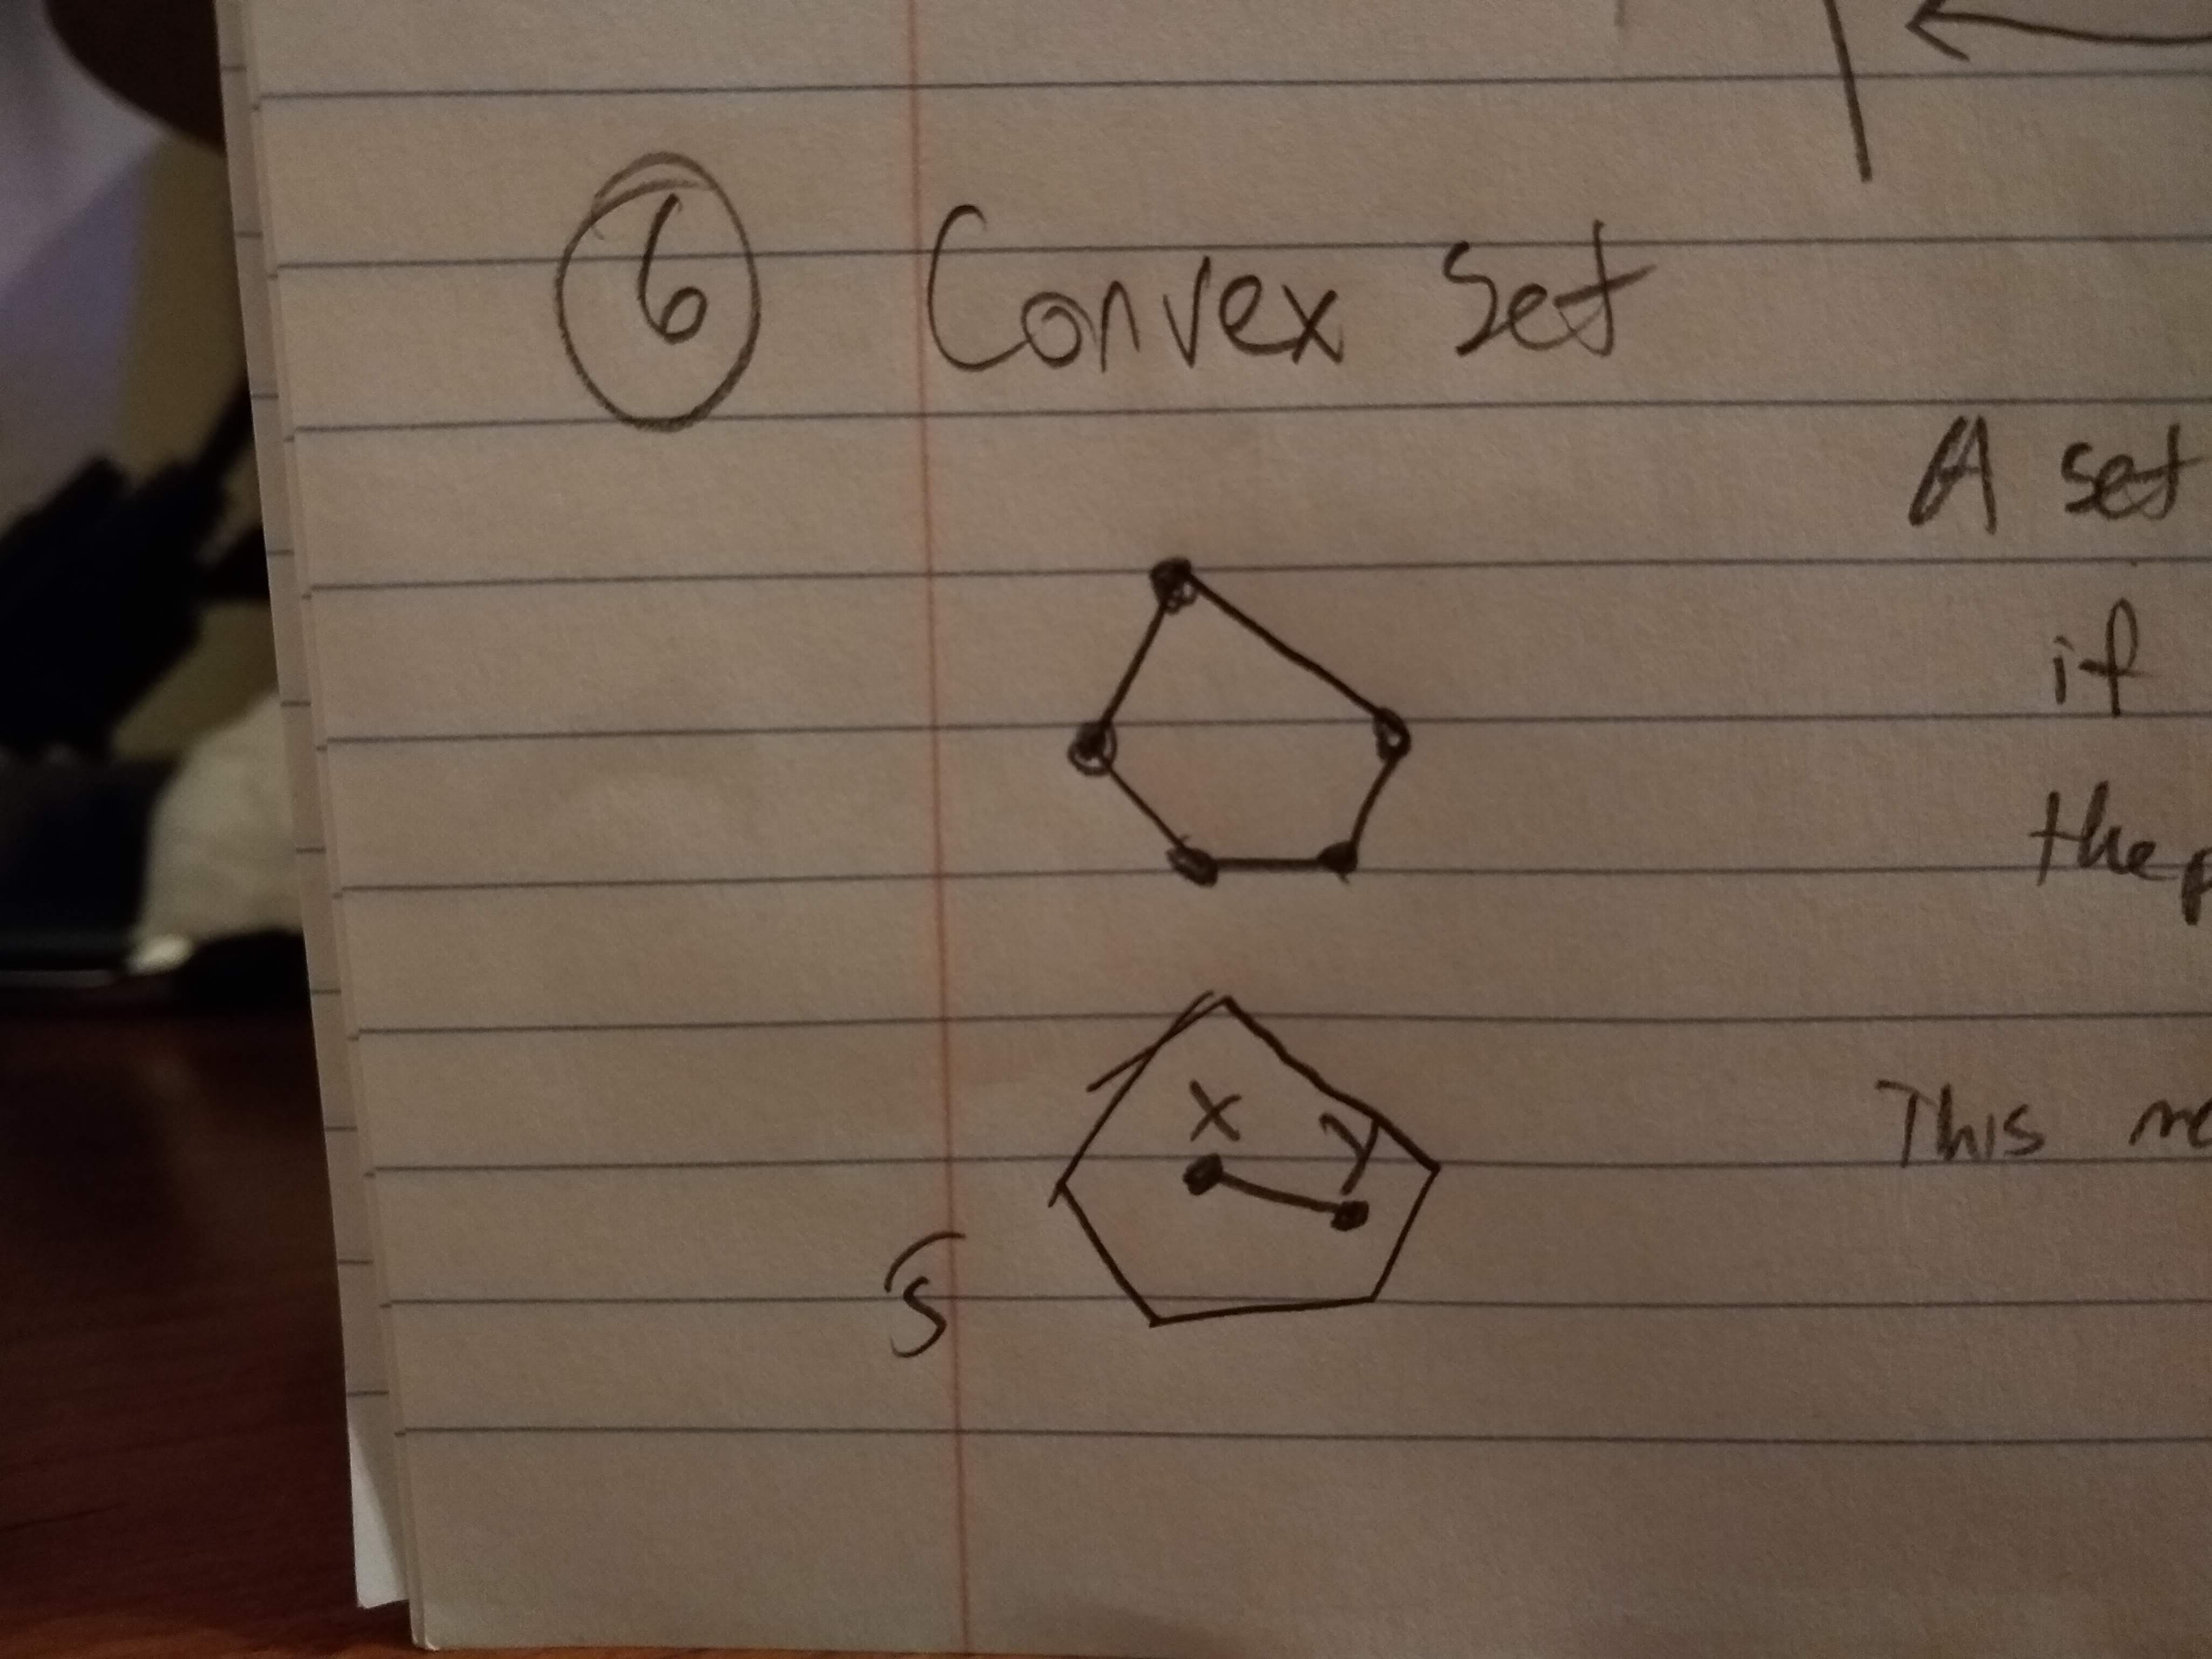
\includegraphics[width=.9\linewidth]{./resources/convex1.jpg}
\end{center}

\subsection{Separating Hyper-plane Theorem}
\label{sec:org220404b}

Let C and D be 2 convex sets that do not intersect. i.e. the sets are
\textbf{disjoint}.

Then there \uline{exists} a vector \(\vec{a} \neq 0\) and a number \uline{b} such that.

$$
a^Tx \leq b \forall x \in C
$$

and

$$
a^T x \geq b \forall x \in D
$$

The Separating Hyper-plane is defined as \({x \colon a^T x = b}\) for sets C, D.

\textbf{This is the theoretical guarantee for ML}


\begin{quote}
vector a is perpendicular to the plane b.
\end{quote}
\section{Why Separating Hyperplane Theorem \& Subspace Segmentation Example (2020/04/07)}
\label{sec:org09c669a}

\subsection{Why is Separating Hyper-plane Theorem true?}
\label{sec:org02d8ed8}
\subsubsection{Math Background}
\label{sec:orgaa7a537}

Let \(x = d - c, \  y = u - d\)
\begin{enumerate}
\item Square of the \$l\textsubscript{2}\$-norm is the inner product
\label{sec:org369e301}
$$
\| x \|_2^2 = \langle x, x \rangle = x^T x
$$


$$
(d - c)^T (d - c) = \| d - c \|_2^2
$$
\item Expansion of Vectors
\label{sec:org5953184}

\begin{equation}
\begin{split}
& \| x + ty \|_2^2\\
= & \langle x + ty, x + ty \rangle\\
= & \| x\|_2^2 + 2t \langle x, y \rangle + t^2 \| y \|_2^2
\end{split}
\end{equation}
\item Derivative of vector products
\label{sec:orgb34d0e7}

$$
\frac{d}{dt}(\| x + ty \|_2^2) = 2 x^T y + 2t  y^T y
$$

$$
\frac{d}{dt}(\| x + ty \|_2^2)|_{t = 0 } = 2 x^T y
$$

$$
\frac{d}{dt} (\| d + t(u - d) - c \|_2^2) |_{t = 0} = 2 (d - c)^T (u - d)
$$
\end{enumerate}

\subsubsection{Separating Hyper-plane Theorem}
\label{sec:orgfc0424f}

C, D are convex disjoint sets. Thus there exists a vecto \(\vec a \neq 0\) and a
number \(b\) such that

$$
a^T x \leq b, \forall x \in C
$$

and

$$
a^T x \geq b, \forall x \in D
$$

\({x: a^T x = b}\) is the separating hyper-plane for C,D.


When \(b = 0\), then inconclusive answer.

\subsubsection{Why is it true?}
\label{sec:org7c4fc92}


\begin{center}
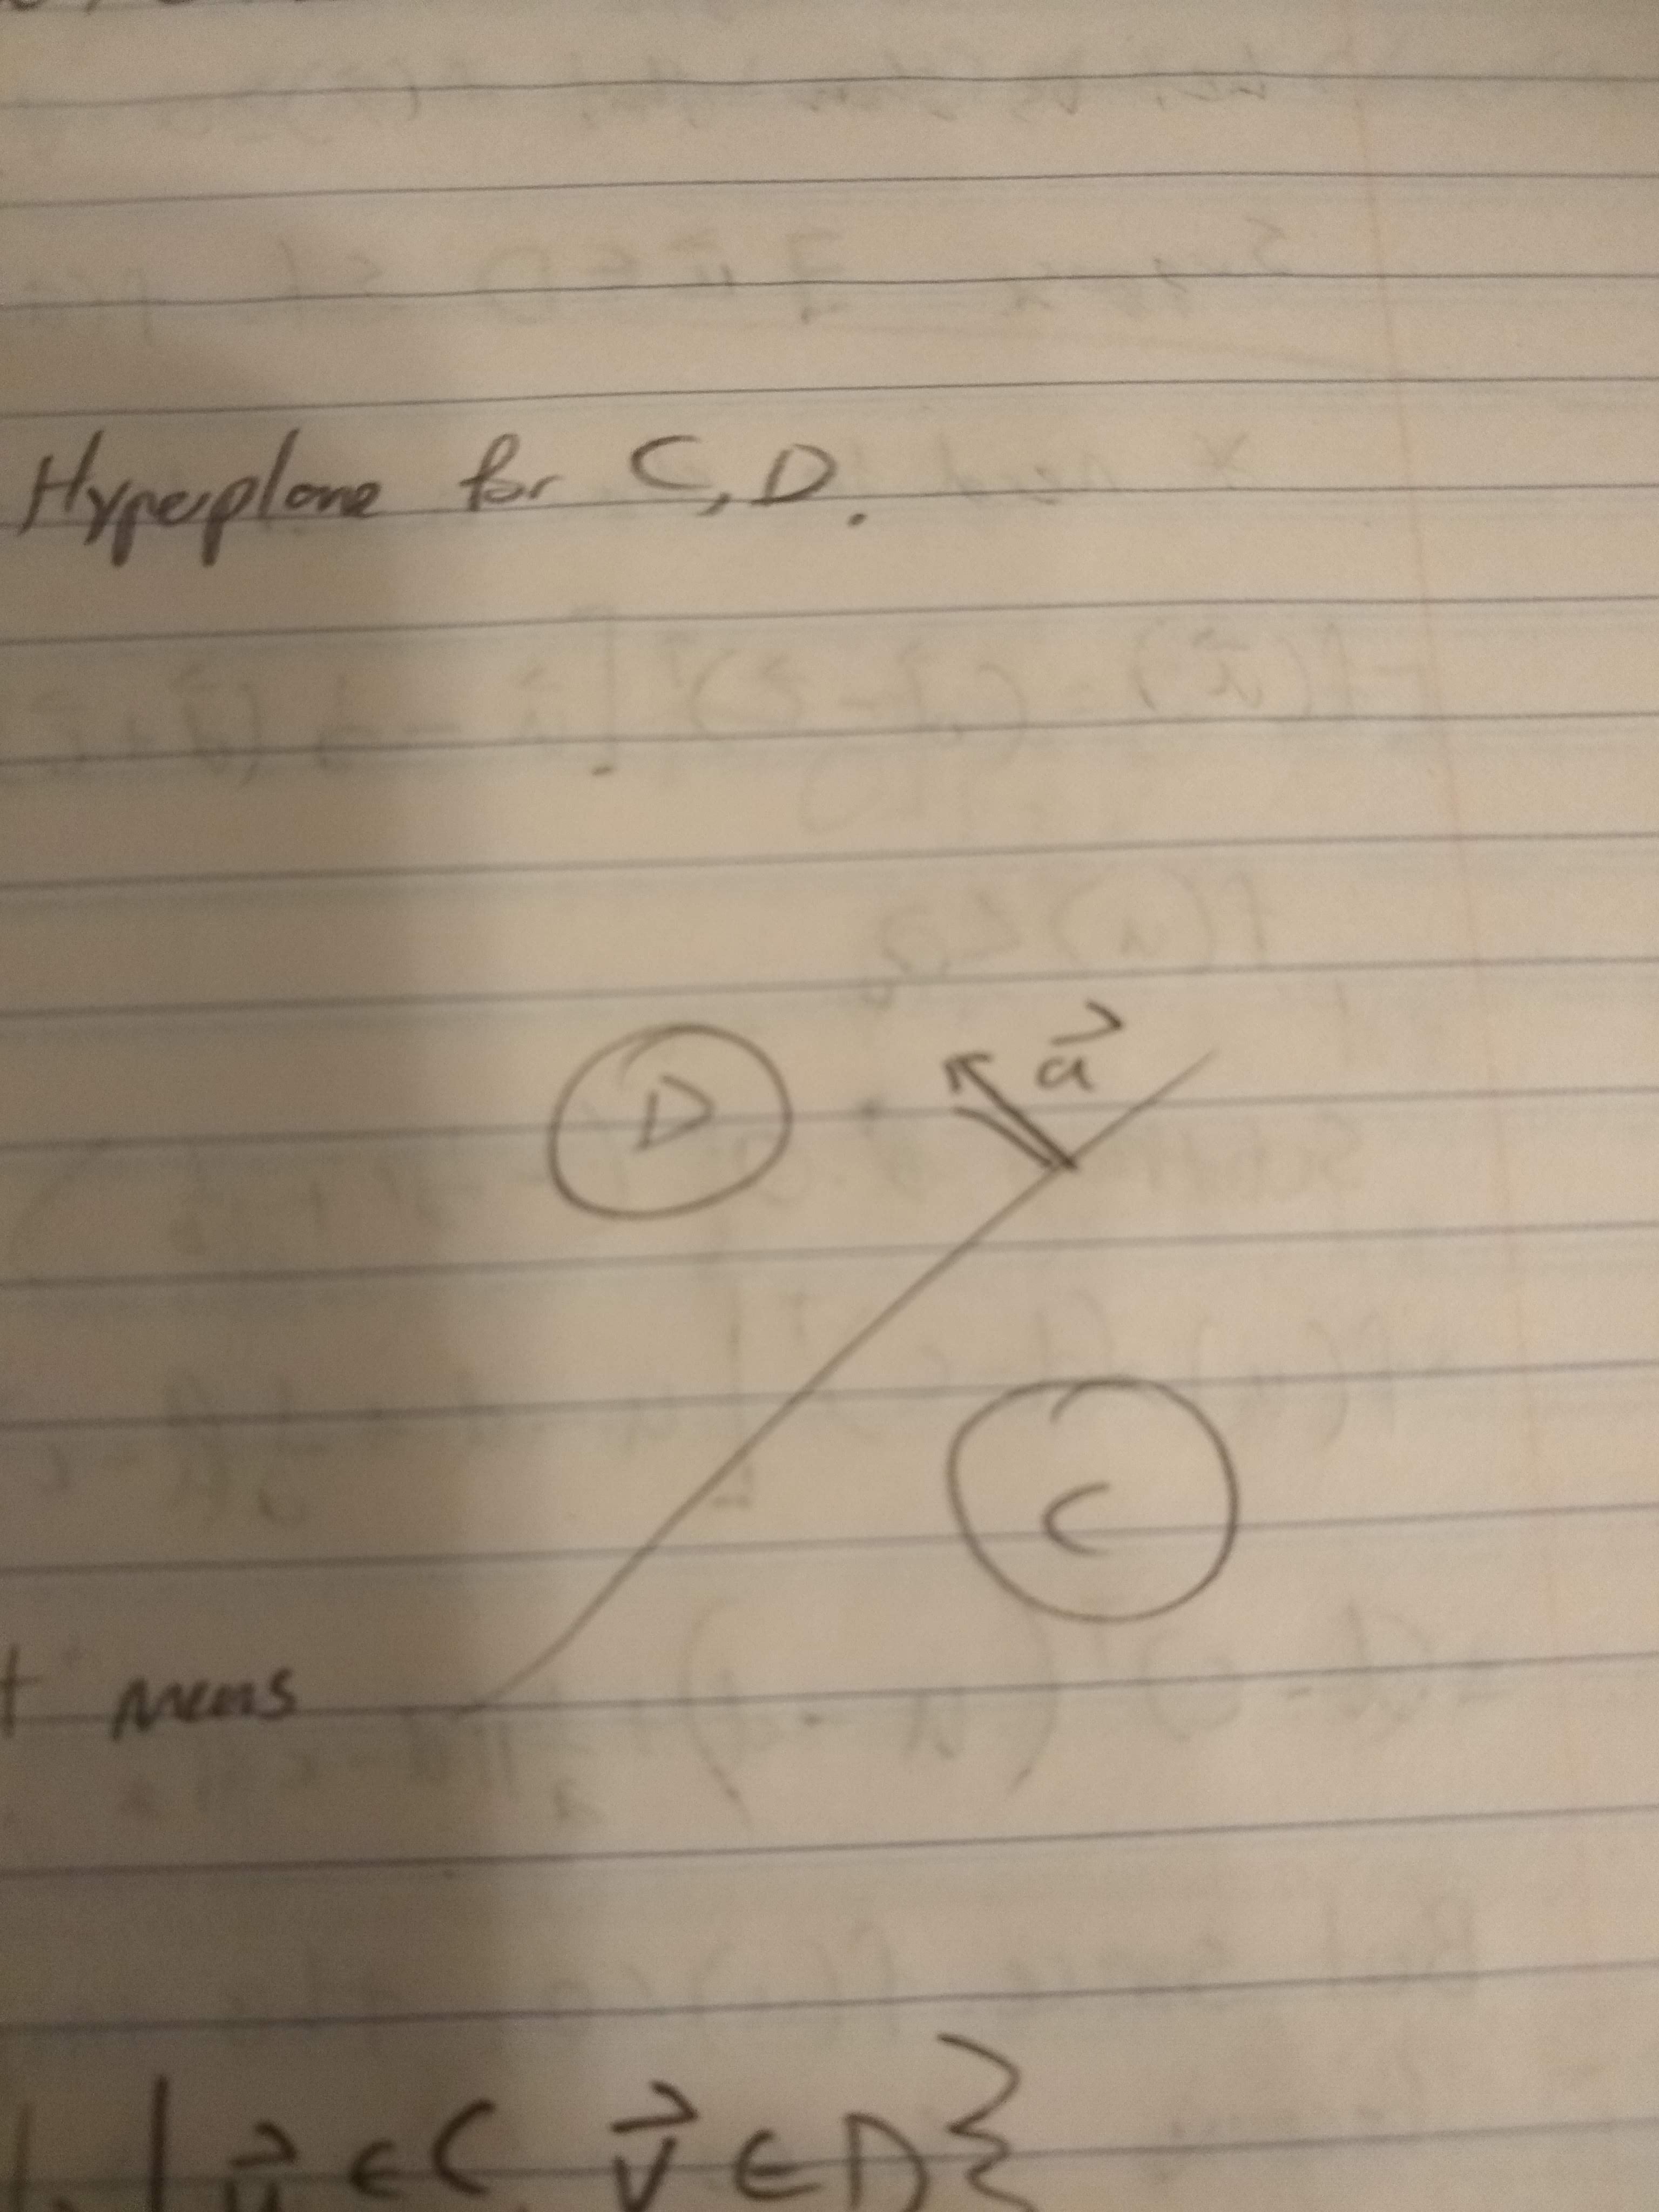
\includegraphics[width=.9\linewidth]{./resources/convex3.jpg}
\end{center}

\begin{equation}
\begin{split}
\vec a^T \vec{x} \leq b \ \text{on side C}\\
\vec{a^T} \vec{x} \geq \ \text{on side D}
\end{split}
\end{equation}

\textbf{Goal}: Prove \(\vec a\) exists as that means a separating hyperplane exists.


$$
dist(C, D) = min{ \| \vec{u} - \vec{v} \|_2 | \vec{u} \in C, \vec{v} \in D} = \|
\vec{c} - \vec{d} \|_2
$$

where \(\| \vec u - \vec v\|_2\) is the euclidean distance.


Let \(\vec a = \vec d - \vec c, \ b = \frac{1}{2}(\| \vec d \|_2^2 - \| \vec c \|_2^2)\)

We will show that

$$
f(\vec x) = a^T x - b
$$

has the property that

$$
f(\vec x) \leq 0, \ \forall \vec x \in C
$$

and

$$
f(\vec x) \geq 0, \ \forall \vec x \in D
$$

Note: \((\vec d - \vec c)^T \frac{1}{2}(\vec d + \vec c) = \frac{1}{2}(\| \vec d
\|_2^2 - \| \vec c \|_2^2)\)

What does showing something mean?

Let us show that \(F(\vec x) \geq 0, \ \forall \vec x \in D\) (Argue by
Contradiction)


Suppose \(\exists \vec{u} \in D\) such that \(f(\vec{x}) < 0\)

$$f(\vec{u}) = (\vec{d} - \vec{c})^T [\vec{u} - \frac{1}{2} (\vec{d} +
\vec{c})]\\
= (\vec{d} - \vec{c})^T \vec{u} - \frac{1}{2}(\| \vec{d}\|_2^2 - \| \vec{c}\|_2^2)$$

\textbf{Subtract 0}

$$
f(u) = (d - c)^T [u - d + \frac{1}{2} \| d - c\|]
$$

\(u - \frac{1}{2}d + \frac{1}{2} c\)

\(u - d + \frac{1}{2} d - \frac{1}{2} c\)

$$
f(u) = (d - c)^T (u - d) + \frac{1}{2} \| d - c \|_2^2
$$

Now we observe that

$$
\frac{d}{dt}(\| d + t (u - d) - c \|_2^2) |_{t = 0} = 2 (d - c)^T (u - d) < 0
$$

and so for some small \(t > 0\),

$$
 \| d + t(u - d) - c \|_2^2 < \| d - c\|_2^2
$$

\(g'(t) < 0\) means decreasing. Thus \(g(t) < g(0)\).

Let's call point \(p = d + t (u - d)\)

Then

$$
\| p - c\|_2^2 < \| d - c\|_2^2
$$

This is a contradiction. Both \(d\) and \(u\) are in set D. Thus by the definition
of convexity, \(p = (1 - t) d + tu\)

D is a convex set so p must also be in D. This situation is impossible since d
is the point in D that is closest to c.

\subsubsection{Example}
\label{sec:orgb0a839a}

Let \(f(\vec x) = a^T x - b\)

\begin{center}
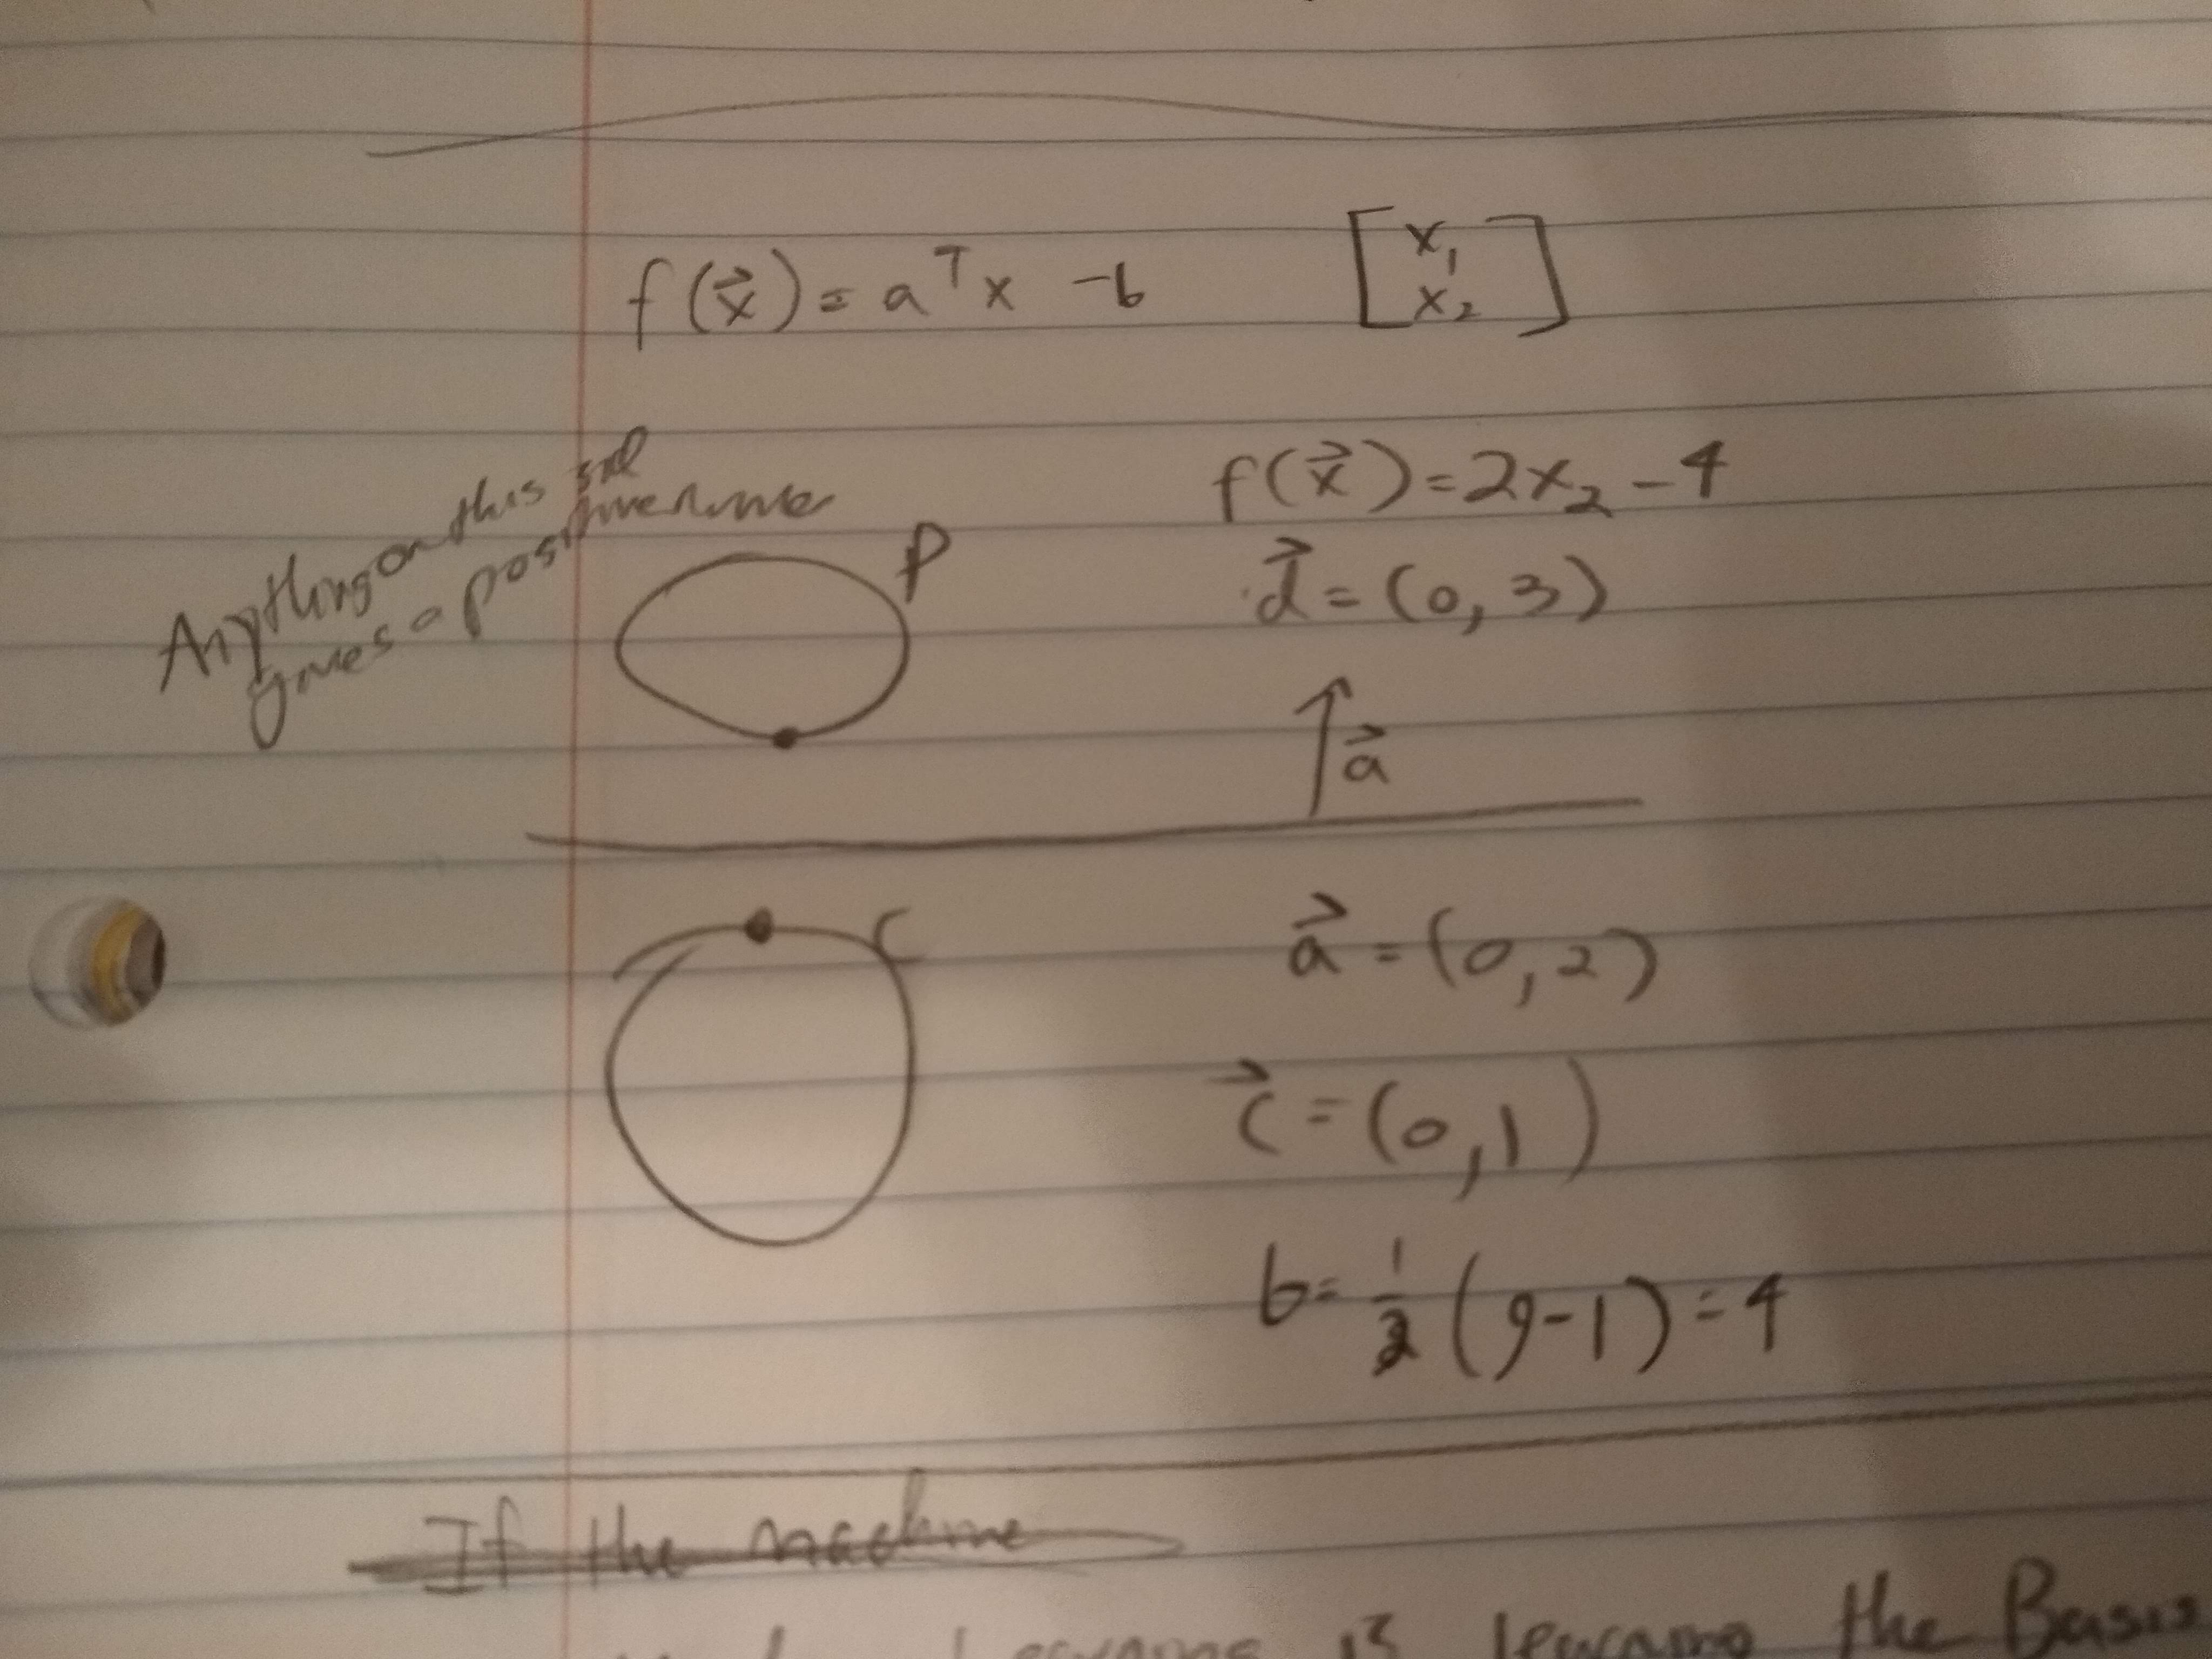
\includegraphics[width=.9\linewidth]{./resources/convex4.jpg}
\end{center}

\subsection{Subspace Segmentation Example}
\label{sec:org3375227}

Machine Learning is learning the Basis A. If we can deduce that a vector \(\vec
x\) is a linear combination of A, then a vector is a subspace of Basis A and we
know that it belongs to A.

$$
V_1 = {(x, y, z) \in R^3 : z = 0}
$$
$$
V_2 = {(x, y, z) \in R^3 : x = 0, y = 0}
$$

\(V_i\) is the affine variety (it is also a Ring, Module)

Apply a Veronase map with degree 2 to lift up from 3 to 6 dimensions.

\(\nu_n \begin{bmatrix} x\\ y\\ z \end{bmatrix} = \begin{bmatrix} x^2\\ y^2\\ z^2\\ xy\\ xz\\ yz \end{bmatrix}, \nu_n: R^3 \to R^6\)

\begin{equation}
\begin{split}
z_1 = (3,4,0), z_2 = (4,3,0),\\
z_3 = (2, 1, 0), z_4 = (1, 2, 0),\\
z_5 = (0, 0, 1), z_6 = (0, 0, 3), z_7 = (0, 0, 4)
\end{split}
\end{equation}

Plug the sample points into the Veronase map to produce a matrix L

$$
L = \begin{bmatrix}
9 & 16 & 4 & 1 & 0 & 0 & 0\\
16 & 9 & 1 & 4 & 0 & 0 & 0\\
0 & 0 & 0 & 0 & 1 & 9 & 6\\
12 & 12 & 2 & 2 & 0 & 0 & 0\\
0 & 0 & 0 & 0 & 0 & 0 & 0\\
0 & 0 & 0 & 0 & 0 & 0 & 0\\
\end{bmatrix} \in R^{6 \times 7}
$$

solve for \(\vec c\), where \(\vec c^T L = \vec 0\)

\(\vec c_1 = \begin{bmatrix} 0\\ 0\\ 0\\ 0\\ 1\\ 0 \end{bmatrix}, \vec c_2 = \begin{bmatrix} 0\\ 0\\ 0\\ 0\\ 0\\ 1 \end{bmatrix}\)

Rank(L) = 4 (since there are 4 linearly independent rows)

\begin{equation}
\begin{split}
q_1(X) = & \vec c^T \nu_n (X)\\
= & xz\\
q_2(X) = & \vec c_2^T \nu_n (X)\\
= & yz
\end{split}
\end{equation}

We have:

\begin{equation}
\begin{split}
q_1(X) = xz & \ \ \ V_1 = (z = 0)\\
q_2(X) = yz & \ \ \ V_2 = (x = 0, y = 0)
\end{split}
\end{equation}

Observe:

\(V_1 \cup V_2 = ((x,y,z) \in R^3: q_1(X) = 0, q_2(X) = 0)\)

Construct the Jacobian matrix

J(Q)(X) = \(\begin{bmatrix} \frac{\partial q_1}{\partial x} & \frac{\partial q_1}{\partial y} & \frac{\partial q_1}{\partial z}\\ \frac{\partial q_2}{\partial x} & \frac{\partial q_2}{\partial y} & \frac{\partial q_2}{\partial z}\end{bmatrix} = \begin{bmatrix} z & 0 & x\\ 0 & z & y \end{bmatrix}\)

\begin{enumerate}
\item When \(z = z_1 = (3, 4, 0), J(Q)(z_1) = \begin{bmatrix} 0 & 0 & 3\\ 0 & 0 & 4 \end{bmatrix}\)

When \(z = z_3 = (2, 1, 0)\), \(J(Q)(z_3) = \begin{bmatrix} 0 & 0 & 2\\ 0 & 0 & 1 \end{bmatrix}\)

The right null space of \(J(Q)(z_1)\) has basis \(\vec b_1 = \begin{bmatrix} 1\\ 0\\ 0 \end{bmatrix}\), \(\vec b_2 = \begin{bmatrix} 0\\ 1\\ 0 \end{bmatrix}\)

\item When \(z = z_5 = (0,0,1)\), \(J(Q)(z_5) = \begin{bmatrix} 1 & 0 & 0\\ 0 & 1 & 0
   \end{bmatrix}\)

When \(z = z_7 = (0, 0, 4)\), \(J(Q)(z_7) = \begin{bmatrix} 4 & 0 & 0\\ 0 & 4 & 0 \end{bmatrix}\)
The right null space of \(J(Q)(z_5)\) has basis \(\vec b = \begin{bmatrix} 0\\ 0\\ 1 \end{bmatrix}\)
\end{enumerate}

\(C = [\vec c_1 | \vec c_2]\)
\section{Sparse Representation \& Problem P0 . P1 (2020/04/14)}
\label{sec:org0955e6d}
\subsection{Big Idea}
\label{sec:org6ee0400}

Your Data is a vector \(x \in R^N\) where all vectors are column
vectors. Each x is s-sparse i.e. each vector has at \textbf{most} \uline{s} non-zero entries. Let s
= 5000. We don't know where the non-zero entries are located.

Let \(\underset{(m \times N)}{A}, \ m < N\)

\(N = 100,000, \ m = 20,000\)

Short + Wide Matrix

\begin{quote}
This is the opposite of the kinds of matrices seen in Linear Regression which
are tall and skinny.
\end{quote}

What if we can design a matrix \(A \in R^{m \times N}\) so that for each s-sparse
\(\vec x \in R^N\), you can store \(\vec y\) instead? (\(A \vec x = \vec y\))

Q: Is there a way to get back \(\vec x\) from \(\vec y\)? We observe \(\vec y\).

A: Yes!

\textbf{Properties of \(A\)}
\begin{itemize}
\item A cannot be the 0 matrix.
\item if \(\vec x_1\) is s-sparse and \(\vec x \neq 0\), what if \(\vec x_1\) is in
\(ker(A)\)? No! that would return \(\vec 0\) which means we cannot reconstruct the
original matrix since there are multiple vectors in Ker(A).
\end{itemize}


\textbf{Using Techniques from 1955}

\begin{enumerate}
\item Is \(\vec x\) the inverse of \(\vec y\) or psuedo-inverse, or Moore-Penrose
inverse, or\ldots{}?
\end{enumerate}

\begin{equation}
\begin{split}
\vec y = & A \vec x\\
A^{\#} \vec y = & A^{\#} A \vec x \ \text{where} \ $A^{\#} A = I$
\end{split}
\end{equation}

Doesn't work! This is because there is no way to guarantee that \(\vec x\) is a
s-sparse vector.

\begin{enumerate}
\item Can we use gradient descent to solve for \(\vec x\) to minimize \(\| \vec y - A \vec x \|_2\)

No! Why?

pick any vector \(\vec v \in Ker(A)\). \(\vec y = A (\vec x + \vec v)\) however,
\((\vec x + \vec v)\) may not be sparse.
\end{enumerate}


New math was needed to solve this problem so it was created in 2005 by Donoho,
Candes, and Tao using the \$l\textsubscript{1}\$-norm instead of the euclidean norm (\(l_2\)).

\subsection{Background}
\label{sec:org2022096}

\textbf{\$l\textsubscript{1}\$-norm}: \(\|x\|_1 = |x_1| + |x_2| + |x_3|\)

\textbf{\$l\textsubscript{2}\$-norm}: \(\|x\| = \sqrt{|x_1|^2 + |x_2|^2 + |x_3|^2}\)

For \(\vec x \in R^n, \ \vec y \in R^N\), then

$$
\| \vec x + \vec y \| \leq \| x \|_1 + \| y \|_1
$$

For a norm to be valid, it must uphold the \textbf{Triangle Inequality}.

\(\vec a\) is one side of a triangle, \(\vec b\) is a second side, third side, \ldots{}

\begin{equation}
\begin{split}
|\vec a + \vec b | \leq |\vec{a}| + |\vec{b}|\\
\| \vec{x} + \vec{y} \|_1 \leq \|\vec{x}\|_1 + \|\vec{y}\|_1\\
\| \vec{x} + \vec{y} \|_2 \leq \|\vec{x}\|_2 + \|\vec{y}\|_2\\
\| \vec{x} + \vec{y} \|_2 \leq \|\vec{x}\|_\infty + \|\vec{y}\|_\infty\\
\end{split}
\end{equation}


It also must be distributive:

If \(\vec x_1 + \vec x_2 = \vec y\), then \((\vec x_1 + \vec x_2) \cdot \vec a =
\vec{y} \cdot \vec{a}\) for any \(\vec a\)

$$
\langle \vec x_1 + \vec x_2, \vec a \rangle = \langle \vec y, \vec a \rangle
\to\\
\langle \vec x_1, \vec a \rangle + \langle \vec x_2, \vec a \rangle = \langle
\vec y, \vec a \rangle
$$

\subsection{Warm-up}
\label{sec:orgc2a503c}

\(A = [\vec a_1 | ... | \vec a_N]\)

\(\| \vec a_j \|_2 = 1 = \langle \vec a_j, \vec a_j \rangle\)


Let \(\vec v \in Ker(A), \ \vec{v} \neq \vec 0, \ \vec v = \begin{bmatrix} v_1 \\ v_2 \\ ... \\ v_N \end{bmatrix}\)

Assume \(\vec a_j\) are unit vectors.

Pick \(i = 3\) observations.

\begin{enumerate}
\item Multiply by 1. Be Sneaky.

\(v_i = v_i \langle \vec a_i, \vec a_i \rangle\)

\item \(\vec v \in Ker(A)\)
\end{enumerate}

\begin{equation}
\begin{split}
& v_1 a_1 + v_2 a_2 + ... + v_n a_n = \vec 0\\
\to & \langle v_1 a_1 + ... + v_N a_N, a_i \rangle = \langle \vec 0, a_i \rangle\\
\to & \langle v_1 a_1, a_i \rangle + ... + \langle v_N a_N, a_i \rangle = \langle \vec 0, a_i \rangle
\end{split}
\end{equation}

Keep \(v_3 \langle a_3, a_i \rangle\) on the left side. Move everything to the
other side. Thus,

$$
v_i = \langle v_i a_i, a_i \rangle = - \sum_{j = 1, j \neq i}^{} v_j \langle a_j, a_i \rangle
$$

Since \(i = 3\), \(v_3 \langle a_3, a_i \rangle = v_i\)

$$| v_i | \leq \sum_{j = 1, j \new i} | v_j | \cdot | \langle a_j, a_i \rangle |$$

What is the absolute value of a single number in \(Ker(A)\)? There is a relation
between \(v_i\) and the rest of the entries in \(\vec v\).

\begin{quote}
Why ``='' becomes \(\leq\)

For example,
if -2 = 3 + (- 5), then
\begin{center}
\begin{tabular}{}
\hline
\end{tabular}
\end{center}
\end{quote}

\subsection{Getting Ready to Formulate the Problem}
\label{sec:orgfc57ea0}

\subsubsection{Problem P0}
\label{sec:org9034598}

Find the s-sparse \(\vec x \in R^N\) such that \(\vec y = A \vec x\).

Ex. Problem 1 HW 1.

Find a 2-sparse vector \(\vec x \in R^8\) such that \(\vec y = A \vec x\).

There are \(8 \choose{2}\) 2-sparse vectors. (28).

Imagine N = 100,000 and s = 5000. Not feasible to try all sparse-vectors.

\subsubsection{Problem P1 (Convex Optimization)}
\label{sec:orga4d106a}

Given \(A \in R^{m \times N}\) and measurement \(\vec y = R^m\), solve the
optimization problem,

$$
\underset{x \in R^N}{min} \| x\|_1
$$

subject to constraint \(y = A \vec x\)

Find a condition on matrix A, so that solving P1 will recover the s-sparse
vector \(x \in R^N\)

\subsection{Null Space Property of Order s}
\label{sec:org24aa92d}
\subsubsection{Setting up Notation}
\label{sec:org0e0c310}
Let \(\vec v \in Ker(A), \ \vec v \neq \vec 0\)

Let the set of indices , where \(\vec v [j] \neq 0\) to be S.

e.g. \(\vec x = \begin{bmatrix} 0\\ 0\\ 2\\ 2\\ 3\\ 0\\ 4 \end{bmatrix}\)

\(S = \{3, 5, 7\}\) (non-zero indices. Also called the support vector of \(\vec v\)).

\(|S| = s\) (number of elements. i.e. sparsity)

\(\bar S = \{1, 2, 4, 6\}\) (complement. i.e zero indices)


$$
\vec v = \begin{bmatrix}1\\ 1\\ 1\\ 1\\ 2\\ -2\\ 2\end{bmatrix}, \vec v_S
= \begin{bmatrix} 0\\ 0\\ 1\\ 0\\ 2\\ 0\\ 2 \end{bmatrix}, \ \vec v_{\bar S}
= \begin{bmatrix} 1\\ 1\\ 0\\ 1\\ 0\\ -2\\ 0 \end{bmatrix}
$$

\(\vec v = \vec v_S + \vec v_{\bar S}\)

\subsubsection{Definition}
\label{sec:org1df2c70}

Let A be a \(m \times N\) matrix.

Let S be a subset or \(\{1,2,3,...,N\}\). Suppose \(N = 50\), and \(S = \{3,5,7\}\)

\begin{enumerate}
\item We say that a matrix A satisfies the null space property with respect to a
set S if
$$
   \| \vec v_S \|_1 < \| \vec_{\bar S} \|, | \forall \vec v \in Ker(A)
   $$
\item If it satisfies the null space property with respect to any set S of size s
where S is a subset of \(\{1,2,3,...,N\}\). \(s < N\)
\end{enumerate}

If a matrix satisfies this property, what does it buy us?

If a matrix A satisfies the Null Space property of order s, then solving problem
P1 will solve P0. i.e. you can recover any s-sparse vector \(\vec x\) from the
measurement \(y\) where \(\vec y = A \vec x\)

\begin{quote}
If A has a small coherence, then it satisfies the Null Space Property of order s.
\end{quote}

Let \(A = [\vec a_1| ... | \vec a_N]\)

$$
\mu_1 = \underset{j \neq k}{max} |\langle \vec a_j, \vec a_k \rangle|
$$

Assume \(\vec a_j\) has \$l\textsubscript{2}\$-norm equal to 1.

\subsubsection{Theorem}
\label{sec:org563a637}

Same assumptions as above.

Suppose \(\mu_1 \cdot s + \mu_1 \cdot (s - 1) < 1\)

The matrix satisfies the Null Space property of order s.

\textbf{Remarks}
\begin{enumerate}
\item \(\mu_1 (2s - 1) < 1\) if true, then A satisfies NSP of order s. It is not a
necessary condition. It is a sufficient condition.
\item From the warm up, if we fix an index i, then for \(\vec v \in Ker(A)\),
\end{enumerate}
\begin{equation}
\begin{split}
|v_i| \leq \sum_{j = 1, j \neq i}^{} |v_j| \cdot |\langle \vec a_j, \vec a_i \rangle|
\end{split}
\end{equation}
\begin{enumerate}
\item Note that \(|v_i|\) is just one term in \(\|v\|_1\) because

$$
   \|v\|_1 = |v_1| + |v_2| + ...
   $$
\end{enumerate}

\subsubsection{Proof}
\label{sec:org143809a}

Given A is an \(m \times N\) matrix. \(A = [\vec a_1 | ... | \vec a_N]\).

Suppose \(\|\vec a_j\| = 1, \ \mu_1 \cdot s + \mu_1 \cdot (s - 1) < 1\)

Show that NSP of order s holds.

i.e.
$$
\|\vec v_S \| < \| \vec v_{\bar S}\|, \forall \vec v \in ker(A)| \{\vec 0\}
$$

and for every set

$$
S \subset \{1,2,3,...,N\} \text{with} |S| = s
$$

Let \(\vec v = Ker(A)\)

\(\vec v = \begin{bmatrix} v_1\\ v_2\\ ...\\ v_n \end{bmatrix}\)

\(A \vec v = v_1 \vec a_1 + ... + v_N \vec a_N = \vec 0\)

Let \(S \subset \{1,2,...,N\}, \ |S| = s\). Pick any \(\vec a_i, i \in S\)

Then \(v_i = v_i \langle \vec a_i, \vec a_i \rangle\). Also, \(v_1 \langle \vec a_i, \vec a_i \rangle + ... + v_N \langle \vec a_N, \vec a_i \rangle = 0\)

\begin{equation}
\begin{split}
\to v_i = v_i \langle \vec a_i, \vec a_i \rangle = - \sum_{j = 1, j \neq i}^{}  v_i \langle \vec a_j, \vec a_i \rangle\\
\to v_i = - \sum_{l \in S}^{} v_l \langle \vec a_l, \vec a_i \rangle - \sum_{j \in S, j \neq i}^{} v_j \langle \vec a_j, \vec a_i \rangle\\
\to |v_i| \leq \sum_{l \in S}^{} |v_l| |\langle \vec a_l, \vec a_i \rangle| + \sum_{j \in S, j \neq i}^{} |v_j| |\langle \vec a_j, \vec a_i \rangle|
\end{split}
\end{equation}

sum over all \(i \in S\) to get

\(\|\vec v_S\|_1 = \sum_{i \in S}^{} |v_i|\)

\begin{quote}
This adds up all the inequalities for one inequality to rule them all.
\end{quote}

\begin{equation}
\begin{split}
\leq & \sum_{i \in S}^{} \sum_{l \in \bar S}^{} |v_l| \cdot |\langle \vec a_l, \vec a_i \rangle| + \sum_{i \in S}^{} \sum_{j \in S, j \neq i}^{} |v_j| \cdot |\langle \vec a_j, \vec a_i \rangle| \\
= & \sum_{l \in \bar S}^{} |v_l| \sum_{i \in S}^{} |\langle \vec a_l, \vec a_i \rangle| + \sum_{j \in S}^{} |v_j| \sum_{i \in S, i \neq j}^{} |\langle \vec a_j, \vec a_i \rangle|\\
\leq & \sum_{l \in S}^{} |v_l| \mu_1 \cdot s + \sum_{j \in S}^{} |v_j| \mu_1 (s - 1)\\
\|\vec v_S\|_1 \leq & \mu_1 \cdot s \|\vec v_{\bar S}\| + \mu_1 (s - 1) \|\vec v_\S\|
\end{split}
\end{equation}

$$
(1 - \mu_1 (s - 1)) \|\vec v_{\bar S}|\ \leq \mu_1 \cdot s \|\vec v_S\|
$$


Since \(\mu_1 (s - 1) + \mu_1 (s) < 1\) by hypothesis, so \(1 - \mu_1 (s - 1) \geq
\mu_1 (s)\)  and hence \(\|\vec v_S\|_1 < \|\vec v_{\bar S}\|_1\)

\subsection{Ways to Solve P1}
\label{sec:orgbf16fd3}

There are 8 algos to solve P1. The worst performing one is Linear programming.

This is one of the Algos

\subsubsection{Algos}
\label{sec:org2066710}

\(A = \begin{bmatrix}1 & 1\end{bmatrix}\)
\(\vec x = \begin{bmatrix} x_1\\ x_2 \end{bmatrix}\)

\(a_{11} = a_{12} = 1\)

\(Q = \begin{bmatrix} \frac{1}{w_1} & 1\\ 0 & \frac{1}{w_2}\end{bmatrix}\)
\begin{enumerate}
\item Minimize \(\|\vec x_1\|\) subject to \(\vec y = A \vec x\)
\end{enumerate}

\begin{equation}
\begin{split}
\vec y = & (A A^T) (A A^T)^{-1} \vec y\\
\vec y = & A (A^T (A A^T)^{-1} \vec y)
\end{split}
\end{equation}

Why not let \(\vec x = (A^T (A A^T)^{-1} \vec y)\)

maybe we can do better.

\(\vec y = A Q A^T (A Q A^T) \vec y\)

Why not let \(\vec x = (Q A^T (A Q A^T)^{-1} \vec y)\)

How to choose Q?

\begin{enumerate}
\item \(min \sum_{i = 1}^{N} W_i x_i^2\) subject to \(\vec y = A \vec x\)

This is not the \$l\textsubscript{1}\$-norm but it would be if \(w_i = \frac{1}{|x_i|}\).

solve 2. then substitute \(w_i\)

\item min: \(w_1 x_1^2 + w_2 + x_2^2\) subject to \(y = a_{11} x_1 + a_{12} x_2\)

\(f(x_1) = w_1 x_1^2 + w_2 (y - x_1)^2\)

\(f'(x_1) = 0\) solve for x\textsubscript{1}

\(2 w_1 x_1 + 2 (y - x_1)(-1)w_2 = 0\)

\(x_1 = \frac{w_2}{w_1 + w_2} y, \ x_2 = \frac{w_1}{w_1 + w_2}v\)
\end{enumerate}


\begin{equation}
\begin{split}
AQA^T = & \begin{bmatrix}1 & 1 \end{bmatrix} \begin{bmatrix} \frac{1}{w_1} & 0 \\ 0 & \frac{1}{w_2} \end{bmatrix} \begin{bmatrix}1\\ 1 \end{bmatrix}\\
= & \frac{w_1 + w_2}{w_1 w_2}
\end{split}
\end{equation}

\begin{equation}
\begin{split}
QA^T(AQA^T)^{-1} y = \begin{bmatrix} \frac{1}{w_1}\\ \frac{1}{w_2} \end{bmatrix} \frac{w_1 w_2}{w_1 + w_2} y
\end{split}
\end{equation}
\section{Sparse Representation pt 2 (2020/04/21)}
\label{sec:orgacffba8}
\subsection{Historical Perspective}
\label{sec:orgfbabc88}
Why is the visual system so powerful? Hypothesis is our brain uses sparse
representation of Visual Data.

Let a picture \(\vec y = c_1 \vec b_1 + ... + c_n \vec b_n\)

so that most \(c_j\) are zero.

Sparse representation used to be called Sparse Coding.

Robust Facial Recognition uses Sparse Subspace Clustering.

Given 19 x 19 images, let \(Y = [\vec Y_1 | ... | \vec Y_{45}], \ \vec y_j \in
R^{361}\)

19 * 19 = 361

Given Y, solve for matrix C
$$
Y = YC, \ diag(C) = \vec 0
$$

Since we don't want \(Y_i = Y_i\), that is why the constraint \(diag(C) = \vec 0\)
is introduced. It ensures that a group of vectors can be a linear combination of
others.

Each column of C is sparse since we want all column vectors to be a linear
combination of a smaller set of columns.


\subsection{Example - Handwritten Digit Recognition}
\label{sec:orga24deda}

Given 28 x 28 images,
Let \(B = [\vec y_1 | ... | \vec y_{4000}]\) where each \(\vec y_j \in R^{784}\)

\begin{itemize}
\item 800 images of 0, 1-800
\item 800 images of 1, 801-1600
\item 800 images of 2, 1601-2400
\item 800 images of 3, 2401-3200
\item 800 images of 8, 3201-4000
\end{itemize}

Let \(\vec f\) be a new image of 2. Solve for X such that \(\vec f = B \vec x\)

Assume \(\vec x\) is 20-sparse.

We would like to see the only \textbf{non-zero} entries at position 1601-2400.

Columns outside the range may be non-zero as well. There is a 95\% probability
that a digit will be 2, 5\% it will be another digit.


\subsubsection{Qualitative Theorem}
\label{sec:org83048f6}
Given \(A^{m \times N}\) with \(m << N\). If A is a Gaussian random matrix, then
with overwhelming high probability, it satisfies some Exact Recovery Condition
for s-sparse Vectors.

For most large undetermined systems of linear equations, the minimal \$l\textsubscript{1}\$-norm
solution is also the sparsest solution.

\begin{quote}
Topics of Research:
\begin{itemize}
\item Theory of Random Matrices
\item Banach Spaces
\end{itemize}
\end{quote}

\subsection{Solving P1 solves P0. Why?}
\label{sec:orgb39a962}
\uline{PO}

Find the s-sparse \(\vec x \in R^N\) such that \(\vec y = A \vec x\).

\uline{P1}

\(A \in R^{m \times N}\) and measurement \(\vec y \in R^m\). Solve optimization
problem,

$$
\underset{x \in R^{N}}{min} \| x\|_1
$$

subject to the constraint \(y = A \vec x\)


Suppose \(\vec y = A \vec x\) and \(\vec y = A \vec z\). Suppose \(\vec x\) is a
sparse vector and \(\vec z\) is \textbf{not}.

We want to show that \(\| \vec x \|_1 < \| \vec x \|_1\) - Null Space property of
order S

\(\| \vec x \|_1 = \| \vec x - \vec z_{S} + \vec z_S \|_1\) - \(\vec z\) restricted
to some Set S. (Subtract 0 so we can use triangle inequality).

Let \(\vec v = \vec x - \vec z, \ \vec v \in Ker(A)\)

\(A (\vec x + \vec z) = A \vec v = \vec 0\)

\begin{subequations}
\label{first:main}
\begin{align}
\|\vec x\|_1 \leq & \|\vec x - \vec z_S\|_1 + \|z_{S}\|_1 \\
= & \| \vec v_S\|_1 + \| \vec z_S \|_1\\
< & \| \vec z_S\|_1 + \| \vec v_{\bar S}\|_1 & \ \text{via Null Space Property}\\
= & \| - \vec z_{\bar S} \|_1 + \| z_S\|_1 & \ \|x_{\bar s}\|_1 = 0 \ \text{since x is sparse}\\
= & \| \vec z \|_1
\end{align}
\end{subequations}



\subsection{Adjoint}
\label{sec:org69cffce}

Let \(T \colon V \to W\). For example, T can be a matrix from \(R^3\) to \(R^2\). In this
case, V is \(R^3\) and W is \(R^2\)

We write \(T^*\) for the adjoint of T.
$$
\forall x \in V, \ \forall y \in W, \ \langle Tx, y \rangle = \langle x, T^* y \rangle
$$

Horrible way to think of it, when T is a matrix, the adjoint is the same as the
transpose.

\textbf{Q}: When A is an orthogonal matrix, what is \(A^* A\)? I

Hint: each column has \$l\textsubscript{2}\$-norm 1, distinct cols are perpendicular.

\textbf{Q}: When A is an orthogonal matrix, why is \(\| Ax \|_2 = \| x \|_2\) for every
 vector x? (This is known as an isometry)

$$
 \| Ax \|_2^2 = \langle Ax, Ax \rangle = \langle x, A^* Ax \rangle = \langle x, x
 \rangle = \| x \|_2^2
 $$

\begin{quote}
This shows that \(\|Ax\|_2^2\) is not too different than \(\|x\|_2^2\)
\end{quote}


\subsection{Restricted Isometry Property (RIP)}
\label{sec:org159f195}

\(A \in R^{m \times N}\) satisfies the restricted isometry property of order s and
level \(\delta_s\) \((0 < \delta_s \leq 1)\)

$$
(1 - \delta_s) \| x\|_2^2 \leq \| Ax\|_2^2 \leq (1 + \delta_s) \| x\|_2^2, \
\forall \ \text{s-sparse} \ x \in R^N
$$

\begin{quote}
Any s columns of the matrix A are \textbf{nearly} orthogonal to each other.
\end{quote}

\textbf{Q}: What can we say about \(|\langle (I - A^* A)x, x \rangle|\) when vector is
s-sparse?

This is a small number.

Let \(u, \ v \in R^N\) and \(S \in \{1,2,3,...,N\}, \ |S| = s\)

What can we say about the following?

$$|\langle u, (I - A* A)v \rangle|$$

We would like to be able to say

\(|\langle u,(I - A^*A)v \rangle| \leq \delta_t \|u\|_2 \|v\|_2\)

\subsubsection{How to think about RIP?}
\label{sec:orgc32d50a}

Suppose A satisfies the restricted isometry property of order s.

\uline{Intuition}: \textbf{Hopefully}, the matrix \(A^* A\) behaves like the Identity Matrix.
\((I - A^*A)\) is small.

If you take some s-sparse vector \(\vec x\) and multiply it by \(I - A^* A\),
hopefully, the resulting vector will also be small.

\subsubsection{Algorithm}
\label{sec:org7631229}

Consider the following vectors,

$$
\vec x_1 = \begin{bmatrix}
10\\ -20\\ 3\\ -4\\ 5\\ -6\\ -7\\ 8\\ 4
\end{bmatrix}, \ \vec x_2 = \begin{bmatrix}
10\\ -20\\ 0\\ 0\\ 0\\ 0\\ -7\\ 8\\ 0
\end{bmatrix}
$$

\uline{Hard Threshold}

\(\tau_s(\vec x)\) is the vector that keeps the s entries that are the largest in
Absolute Value.

Example: When \(s = 4, \ \tau_s(\vec x_1) = \vec x_2\)

\(\tau_s (\cdot)\) is an operator that takes a vector and will output a sparse vector.


\begin{subequations}
\label{first:main2}
\begin{align}
\vec u_n = & \vec x_n + A^* (\vec y - A \vec x_n), \ \text{where} \ \vec y = A \vec x\\
= & \vec x_n + (A^* A \vec x - A^* A \vec x_n)\\
= & (I - A^* A)\vec x_n + A^* A \vec x
\end{align}
\end{subequations}


\begin{itemize}
\item expect \(\vec u_n\) close to \(\vec x\)
\item however, \(\vec u_n\) may not be sparse. Thus use \(\tau_s(\cdot)\)

\uline{Iterative Hard Thresholding}

$$
  \vec x_{n + 1} = \tau_x (\vec x_n + A^* (\vec y - A \vec x_n))
  $$
\end{itemize}
\subsection{Operator Norm}
\label{sec:org5933cfb}

\(\| A \| = \underset{x \neq 0}{max} \frac{\| Ax \|_2}{\| x \|_2}\)

How much influence does A have on a vector x? Shrink, stretch, compress?

Describes how big a matrix is. If A is 2 x 3, then take \(\vec x \in R^3, \ x
\neq 0\)

What is

$$
\| A \| = max\{ \| Ax \|_2 \colon \| x \|_2 = 1 \}
$$

\subsubsection{Inner Product}
\label{sec:org51d19f9}

Let A be a matrix . The inner product of two vectors \(Ax\) and \(y\) has this
property,

$$| \langle Ax, y \rangle | \leq \| A\| \cdot \|x\|_2 \|y\|_2$$

Where \(\|A\|\) is the operator norm of A.

By Cauchy-Schwartz Inequality,

$$
\|\langle Ax, y \rangle\| \leq \|Ax\|_2 \cdot \|y\|
$$

By def,

$$
\|Ax\| \leq \|A\| \cdot \|x\|_2
$$

Thus,

$$
\|\langle Ax, y \rangle\| \leq \|A\| \cdot \|x\|_2 \cdot \|y\|_2
$$

\section{Sparse Representation Pt 3 (2020/04/28)}
\label{sec:orge2cf396}

\subsection{Expanding on RIP}
\label{sec:org01c2325}

Expanding upon \hyperref[sec:org159f195]{RIP}

Any S columns of the matrix A are nearly orthogonal to each other.

\subsection{Expanding on IHT}
\label{sec:org4441057}
Expanding upon the \hyperref[sec:org7631229]{IHT Algorithm},

\(\tau_x ( \cdot )\) is an \uline{non-linear operator} that outputs a sparse matrix. The
operator is non-linear because it does not \emph{change} the dimensions on the
vector. i.e. \(R^n \to R^n\). You will not be able to find a matrix that will return the same output as this operator.

\(\tau_s (\vec x_1) = x_2\)

Which means both \(\vec x_1\) and \(\vec x_2\) have an inner product.

The IHT algorithm is described below:

\begin{subequations}
\label{first:main2}
\begin{align}
\vec u_n = & \vec x_n + A^* (\vec y - A \vec x_n), \ \text{where} \ \vec y = A \vec x\\
= & \vec x_n + (A^* A \vec x - A^* A \vec x_n)\\
= & (I - A^* A)\vec x_n + A^* A \vec x
\end{align}
\end{subequations}


We expect \(\vec u_n\) is close to \(\vec x\).

What does it mean for a matrix A to be small? matrix A is small when \(A \vec x\)
is small.

\subsection{IHT Proof}
\label{sec:orgfdc72b6}

Suppose A satisfies RIP of order 3s with

$$
\delta_{3s} < \frac{1}{2}
$$

\(\delta_{3s}\):  relaxation.

\(3s\): every 3s columns need to be orthogonal

\(\frac{1}{2}\): how far from orthogonality the difference can be.

Then the sequence \(\{\vec x_n\}\) defined by

$$
\vec x_{n + 1} = \tau_S (\vec x_n + A^* (\vec y - A \vec x_n))
$$

will converge to \(\vec x\)

\begin{quote}
Note: 3s-sparse vectors and s-sparse vectors are \textbf{not} the same.
\end{quote}

\subsubsection{How to think about this?}
\label{sec:orgdcf21eb}

\(u\) and \(v\) are 2s-sparse.

Let \(S_1\) be the support of \(u\). Meaning \(S_1 = \{j: u(j) \neq 0\}\)

Let \(S_2\) be the support of \(v\).

Let \(S\) be the union of \(S_1\) and \(S_2\). Assume \(|S| = 3s\)

If A satisfies RIP of order 3s. Then

\(|\langle u, (I - A^* A)v \rangle| \leq \delta_{3s} \|u\|_2 \cdot \|v\|_2\)

\begin{subequations}
\label{first:main}
\begin{align}
\|\langle u, (I - A^* A) \rangle\| & \leq  \|u\|_2 \ \|v(I - A^* A)\|_2\\
& \leq \|u\|_2 \ \|v \delta_{3s}\|_2\\
& \leq \delta_{3s} \ \|u\|_2 \ \|v\|_2
\end{align}
\end{subequations}

\subsubsection{Explanation: Why is the theorem true?}
\label{sec:orgcfd637c}

We want to find a constant \(\lambda, \ 0 \leq \lambda < 1\) s.t.

$$
\|x_{n+1} - x\|_2 \leq \lambda \|x_n - x\|_2, \ \forall \ n = 1,2,3,...
$$

Why?

\begin{equation}
\begin{split}
\|x_4 - x\|_2 \leq & \lambda \|x_3 - x\|_2\\
\|x_3 - x\|_2 \leq & \lambda \|x_2 - x\|_2\\
\|x_2 - x\|_2 \leq & \lambda \|x_1 - x\|_2
\end{split}
\end{equation}

Therefore,

\begin{equation}
\begin{split}
\|x_4 - x\|_2 \leq \lambda^{n - 1} \ \|x_1 - x\|_2
\end{split}
\end{equation}


In general,

\begin{equation}
\begin{split}
\|x_{n + 1} - x\|_2 \leq \lambda^{n - 1} \ \|x_1 - x\|_2
\end{split}
\end{equation}

as \(n \to \infty, \ \lambda \to 0\) (because \(\lambda < 1\))


$$
\vec x_{n + 1} = \tau_S (\vec x_n + A^* (\vec y - A \vec x_n))
$$

and

$$
x_{n + 1} = \tau_S (u_n)
$$

\(x_{n + 1}, \ x\) are s-sparse.

\uline{Key Observation}: Which one (\(x_{n + 1}\) or \(x\)) is a better approximation to
\(u_n\)?

\(x_{n + 1}\)

Thus,

\begin{equation}
\begin{split}
\|u_n - x_{n + 1}\|_2^2 \leq \|u_n - x\|_2^2
\end{split}
\end{equation}

\textbf{What is \(u_n - x\)?}

\begin{subequations}
\label{first:second}
\begin{align}
u_n - x = & x_n + A^* A (x - x_n) - x\\
= & (I - A^* A) x_n + (A^* A - I)x\\
= & (I - A^* A) (x_n - x)
\end{align}
\end{subequations}

\textbf{What is \(u_n - x_{n + 1}\)?}

\begin{subequations}
\label{first:third}
\begin{align}
\|u_n - x_{n + 1}\|_2^2 = & \|u_ - x_{n + 1} - (x - x)\|_2^2, & \text{subtract 0}\\
= & \|(u_n - x) - (x_{n + 1} - x)\|_2^2, & \text{square of l2 norm os inner product}\\
= & \langle (u_n - x) - (x_{n + 1} - x), (u_n - x) - (x_{n+1} - x) \rangle\\
= & \|u_n - x\|_2^2 - 2 \langle u_n - x, x_{n + 1} - x \rangle + \|x_{n + 1} - x\|_2^2
\end{align}
\end{subequations}

From the above two formulas, we getattr

\begin{equation}
\begin{split}
-2 \langle u_n - x, x_{n + 1} - x \rangle + \|x_{n + 1} - x\|_2^2 \leq 0
\end{split}
\end{equation}

This is the same as

$$
\|x_{n + 1} - x\|_2^2 \leq 2 \langle u_n - x, x_{n + 1} - x \rangle
$$

What is \(u_n - x\)?

$$
u_n - x = (I - A^* A) (x_n - x)
$$

$$
\langle u_n - x, x_{n + 1} - x \rangle = & \langle (I - A^* A)(x_n - x), x_{n +
1} - x \rangle
$$


Thus,

$$
u = x_{n - x}, \ v = x_{n + 1} - x
$$


Why? \(x_n - x\) is 2s-sparse and \(x_{n + 1} - x\) is also 2s-sparse.


We have shown that

$$
\langle u_n - x, x_{n + 1} - x \rangle \leq \delta_{3s} \|x_{n} - x\|_2 \cdot \|x_{n + 1} - x\|_2
$$


\begin{equation}
\begin{split}
\|x_{n + 1} - x\|_2^2 \leq & 2 \delta_{3s} \|x_{n} - x\|_2 \cdot \|x_{n + 1} - x\|_2\\
\|x_{n + 1} - x\|_2 \leq & 2 \delta_{3s} \cdot \|x_n - x\|_2
\end{split}
\end{equation}

The hypothesis is \(\delta_{3s} < \frac{1}{2}\) and so \(0 \leq \lambda < 1\)

\begin{equation}
\begin{split}
\|x_{n + 1} - x\|_2 \leq \lambda \|x_n - x\|_2
\end{split}
\end{equation}

Explanation succeeded

\subsection{Convex Functions}
\label{sec:org678ea73}

Pick any norm, \(\|\cdot\|_1, \ \|\cdot\|_2\)

We have the triangle inequality

\begin{equation}
\begin{split}
\|x + y\| \leq \|x\| + \|y\|
\end{split}
\end{equation}

Suppose we define \(f(x) = \|x\|\) for any \(x \in R^d\) and \(0 \leq \theta \leq 1\).

\begin{equation}
\begin{split}
f(\theta x = (1 - \theta) y) = & \|\thetax + (1 - \theta)y\| \leq \|\theta x\| + \|(1 - \theta) y\|\\
= & \theta \|x\| + (1 - \theta) \|y\|
\end{split}
\end{equation}



Hence, \(f(\theta x + (1 - \theta) y) \leq \theta f(x) + (1 - \theta) f(y)\) so
\(f(x)\) is a convex function.

\subsection{Convex Optimization}
\label{sec:org480da42}

Suppose you have a convex function defined over a convex set C, and you want to
find the minimum of the function over the set C.

What do you have? A convex optimization problem!

Let \(f(x)\) be a convex function over \(R^d\). Minimize \(f(x)\) subject to \(Ax = b\).

The domain D is the set of \(x \in R^d\) such that \(Ax = b\).

If \(Ax = b\), and \(Ay = b\), then \(A(tx + (1 - t)y) = b\). Thus D is a convex set.

If x and y are both in D, then the line segment joining x and y is entirely in D.

\subsection{Why is convex optimization important?}
\label{sec:org83ec00c}

Fundamental property of Convex optimization:

Any \uline{\_local minimum} of a convex function \(f\) over a convex set C \textbf{must} also be
a \uline{global minimum} of \(f\) over C.
\section{Gradient Descent (2020/05/05)}
\label{sec:orga0cf17c}

\subsection{Method of Steepest Descent}
\label{sec:org04e285f}

Let \(x \in R^3, \ y \in R^3\). these are column vectors in \(R^3\)

\begin{equation}
\begin{split}
f(x) = & f(x_1, x_2, x_3)\\
f(y) = & f(y_1, y_2, y_3)\\
G(y) = & G(y_1, y_2, y_3)\\
\end{split}
\end{equation}

\(\nabla f(x)\) is a gradient vector. The convention is that the gradient is a
\textbf{row} vector.

\(G(y) = f(y) - \nabla f(x) y\)

\begin{equation}
\begin{split}
\nabla f(x) \equiv & (\frac{\partial f}{\partial x_1}, \frac{\partial f}{\partial x_2}, \frac{\partial f}{\partial x_3})\\
\nabla f(x) y = & \frac{\partial f}{\partial x_1} y_1  + \frac{\partial f}{\partial x_2} y_2 + \frac{\partial f}{\partial x_3} y_3\\
= & \begin{bmatrix}
\frac{\partial f}{\partial x_1} & \frac{\partial f}{\partial x_2} & \frac{\partial f}{\partial x_3}
\end{bmatrix} \begin{bmatrix}
y_1\\ y_2\\ y_3
\end{bmatrix}
\end{split}
\end{equation}

\subsubsection{Warm Up}
\label{sec:orgab128bf}

\(\nabla G(y) = \nabla [f(y) - \nabla f(x) y] = \nabla f(y) - \nabla f(x)\)


We assume
$$
f(x) - f(y) - \nabla f(y) (x - y) \leq \frac{b}{2} \|x - y\|_2^2
$$

\begin{quote}
This assumption drives from Taylor's Theorem  where the Hessian Matrix (Matrix
of 2ND Derivatives) is bounded by the largest Eigenvalue.
\end{quote}

For any given x, consider the function

$$
G(y) = f(y) - \nabla f(x) y
$$

G is convex.

\(G(y) \equiv G_x (y)\) because G depends on x.

Suppose x is the minimizer of \(G(y)\)

$$
G(x) \leq G(y - \frac{1}{b} \nabla G(y))
$$

and

$$
\nabla G(y) = \nabla [f(y) - \nabla f(x) y] = \nabla f(y) - \nabla f(x)
$$

We assume \(f(x)\) is \(C^1\) and satisfies the condition:

$$
\forall x, \ y, \ f(x) - f(y) \leq \nabla f(y) (x - y) + \frac{b}{2} \|x - y\|_2^2
$$

\begin{quote}
\(C^1\): continuously differentiable.
What happens y = x?
$$
\nabla G(x) = \nabla f(x) - \nabla f(x) = 0
$$

meaning that its a minimum, which is a global minimum because G is converse.
Thus explaining \uline{why} x is a minimizer?
\end{quote}

\(G(y - a) - G(y)\)

Let \(x = y - a, a = \frac{1}{b} \nabla G(y)\)

\begin{quote}
When making an assumption, make an assumption that allows you to learn something interesting.
\end{quote}

\begin{equation}
\begin{split}
& \leq \nabla G(y)(x - y) + \frac{b}{2} \|x - y\|_2^2\\
& = \nabla G(y)(-a) + \frac{b}{2} \|x - y\|_2^2\\
& = \nabla G(y)(- \frac{1}{b} \nabla G(y)^T) + \frac{b}{2} \ \frac{1}{b^2} \|\nabla G(y)\|_2^2
\end{split}
\end{equation}

We just demonstrated

\begin{equation}
\begin{split}
& G(y - \frac{1}{b} \nabla G(y)) - G(y)\\
& \leq \nabla G(y)(- \frac{1}{b} \nabla G(y)^T) + \frac{b}{2} \ \frac{1}{b^2} \|\nabla G(y)\|_2^2
\end{split}
\end{equation}

\subsubsection{Proving Gradient Descent}
\label{sec:org5d0ce5e}


$$
\nabla G(y) = \nabla [f(y) - \nabla f(x) y] = \nabla f(y) - \nabla f(x)
$$

\begin{subequations}
\label{first:main}
\begin{align}
\to & f(x) - f(y) - \nabla f(x) (x - y)\\
= & f(x) - \nabla f(x) x - (f(y) - \nabla f(x) y)\\
= & G(x) - G(y)\\
= & G(y - \frac{1}{b} \nabla G(y)) - G(y)\\
\leq & \nabla G(y)(- \frac{1}{b} \nabla G(y)^T) + \frac{b}{2} \ \frac{1}{b^2} \|\nabla G(y)\|_2^2\\
= & - \frac{1}{2b} \|\nabla G(y)\|_2^2\\
= & - \frac{1}{2b} \|\nabla f(x) - \nabla f(y)\|_2^2
\end{align}
\end{subequations}

[g] says

$$
f(x) - f(y) - \nabla f(x) (x - y) \leq - \frac{1}{2b} \|\nabla f(x) - \nabla f(y)\|_2^2
$$

We define a sequence of vectors

$$x_{k + 1} = x_k - \frac{1}{b} g_k$$

\(x_{k + 1} = x_k - \frac{1}{b} \nabla f(x_k)\)

Using \(\frac{1}{b}\) is \textbf{Bold}. The old style updated the step at each iteration
which results in less iterations but more compute.

\(h = \frac{1}{b}\)

Let us write

\begin{equation}
\begin{split}
d_k = & x_k - x^* & \text{How far the current estimate is from the minimum}\\
\delta_k = & f(x_k) - f(x^*) & \text{Actual Error}
\end{split}
\end{equation}

Thus,

$$
d_{k + 1} = x_{k + 1} - x^*
$$

Apply [g] with \(x = x_k, \ y = x^*\)

\begin{equation}
\begin{split}
& f(x_k) - f(x^*) - g_k^T (x_k - x^*) \leq - \frac{1}{2b} \|\nabla f(x_k) - \nabla f(x^*)\|_2^2\\
& \to \delta_k \leq g_k^T d_k - \frac{1}{2b} \|g_k\|_2^2
\end{split}
\end{equation}

because \(g_k = \nabla f(x_k)\) and \(d_k = x - x^*\)

G: scalar
everything else: vector

\uline{Look Closer}!


$$x_{k + 1} - x_k = - \frac{1}{b} g_k$$ <= Using \(x_{k + 1} - \frac{1}{b} g_k\)

\(g_k = -b (x_{k + 1} - x_k)\)

\begin{subequations}
\label{first:main2}
\begin{align}
\delta_k \leq & g_k^T d_k - \frac{1}{2b} \|g_k\|_2^2\\
= & -b(x_{k + 1} - x_k)^T d_k - \frac{b}{2} \|x_{k + 1} - x_k\|_2^2\\
= & - \frac{b}{2}(\|x_{k + 1} - x_k \|_2^2 + 2(x_{k + 1} - x_k)^T d_k)\\
= & - \frac{b}{2}(\|d_{k + 1} - d_k \|_2^2 + 2(d_{k + 1} - d_k)^T d_k)\\
= & \|d_{k + 1} - d_k\|_2^2 + 2(d_{k + 1} - d_k)^T d_k\\
= & (\langle d_{k + 1}, d_{k + 1} \rangle - 2 \langle d_{k + 1}, d_k \rangle + \langle d_k, d_k \rangle) + (2 d_{k + 1}^T d_k - 2d_k^T d_k)\\
= & (\langle d_{k + 1}, d_{k + 1} \rangle - 2 \langle d_{k + 1}, d_k \rangle + \langle d_k, d_k \rangle) + (2 \langle d_{k + 1}, d_k \rangle - 2 \langle d_k, d_k \rangle)\\
= & - \frac{b}{2}(\langle d_{k + 1}, d_{k + 1} \rangle - \langle d_k, d_k \rangle)\\
= & \frac{b}{2}(\|d_k\|_2^2 + \|d_{k + 1}\|_2^2)\\
\end{align}
\end{subequations}


To summarize,

$$
\delta_k \leq \frac{b}{2} (\|d_k\|_2^2 - \|d_{k + 1}\|_2^2)
$$

$$
\sum_{i = 1}^{n} \delta_i \leq \frac{b}{2} (\|d_0\|_2^2 - \|d_{n}\|_2^2 \leq
\frac{b}{2} \|d_0\|_2^2
$$

What do we know about convergent series?

If \(\sum_{k = 1}^{\infty} \delta_k\) is convergent, then \(\delta_k \to 0\) as \(k
\to \infty\)

\subsection{Global Convergence}
\label{sec:orgace1f76}

Start with any \(x_0\). We define the sequence of vectors

$$x_{k + 1} = x_k - \frac{1}{b} g_k$$

\(x_{k + 1} = x_k - \frac{1}{b} \nabla f(x_k)\)

Then, \(f(x_k) - f(x^*) \to 0\) as \(k \to \infty\)

We can pick N as large as we want,

$$
\sum_{k = 0}^{N} \delta_k \leq \frac{b}{2} \|d_0\|_2^2
$$

Recall that \(g_k \equiv \nabla f(x_k)\) and \(g_{k + 1} \equiv \nabla f(x_{k + 1})\)

We can also show that \(\|g_{k + 1}\| \leq \|g_k\|\)

The length of the gradient vectors are monotone decreasing.

We've shown that

$$
f(x) - f(y) - \nabla f(x) (x - y) \leq - \frac{1}{2b} \|\nabla f(x) - \nabla f(y)\|_2^2
$$

Similarly,


$$
f(y) - f(x) - \nabla f(y) (y - x) \leq - \frac{1}{2b} \|\nabla f(x) - \nabla f(y)\|_2^2
$$

Summing the above inequalities yields

$$-\nabla f(x) (x - y) - \nabla f(y) (y - x) \leq - \frac{1}{b} \|\nabla f(x) -
\nabla f(y)\|_2^2$$

which means,

$$
(\nabla f(x) - \nabla f(y)) (x - y) \geq \frac{1}{b} \|\nabla f(x) - \nabla
f(y)\|_2^2 \ \ \ \text{**}
$$

Let \(x = x_{k + 1}, \ y = x_k\). Then, from (**),

$$
(x_{k + 1} - x_k)^T (g_{k + 1} - g_k) \geq \frac{1}{b} \|g_{k + 1} - g_k\|_2^2
$$

But \(x_{k + 1} = x_k - \frac{1}{b} g_k\) so that

$$
-\frac{1}{b} (g_k)^T (g_{k + 1} - g_k) \geq \frac{1}{b} \|g_{k + 1} - g_k\|_2^2
$$

\begin{subequations}
\label{first:mythird}
\begin{align}
-\frac{1}{b} (g_k)^T (g_{k + 1} - g_k) \geq & \frac{1}{b} \|g_{k + 1} - g_k\|_2^2\\
- (g_k)^T (g_{k + 1} - g_k) \geq & \|g_{k + 1} - g_k\|_2^2\\
- g_k^T g_{k + 1} + g_k^T g_k) \geq & \|g_{k + 1} - g_k\|_2^2\\
\langle g_k, g_k \rangle - \langle g_k, g_{k+1} \rangle \geq & \|g_{k + 1} - g_k\|_2^2\\
\langle g_k, g_k \rangle - \langle g_k, g_{k+1} \rangle \geq & \langle g_{k + 1}, g_{k + 1} \rangle - 2 \langle g_{k + 1}, g_k \rangle + \langle g_k, g_k \rangle\\
\langle g_k, g_{k+1} \rangle \geq & \langle g_{k + 1}, g_{k + 1} \rangle\\
\|g_{k+1}\|_2^2 \leq & g_{k+1}^T g_k
\end{align}
\end{subequations}


\begin{subequations}
\label{first:main}
\begin{align}
\|g_{k + 1}\|_2^2 \leq & g_{k + 1}^T g_k\\
\leq & \|g_{k + 1}\| \|g_k\| & \text{By Cauchy-Schwartz}
\end{align}
\end{subequations}


That means, \(\|g_{k+1}\| \leq \|g_k\|\), which is the desired conclusion


\subsection{About Gradient Descent}
\label{sec:orgf4b28e2}

Gradient Descent is \emph{not} a single method. It is a large collection of methods.

\begin{enumerate}
\item Steepest Descent with a constant step size
$$x_{k + 1} = x_k - h \nabla f(x_k)$$

\item Use a different step size at each iteration
$$x_{k + 1} = x_k - \alpha_k \nabla f(x_k)$$
\end{enumerate}


\subsubsection{Example}
\label{sec:org0c451f9}

Select \(\alpha_k\) to minimize \(f(x_k - d_k g_k)\), where \(g_k = \nabla f(x_k)\).
Lots of algorithms to choose \(\alpha_k\)

We assume \(f(x)\) is \(C^1\) and satisfies

$$
f(x) - f(y) \leq \nabla f(y)(x - y) + \frac{b}{2} \|x - y\|_2^2
$$

If we assume f is convex, differentiable, and its gradient vector satisfies the
Lipshitz Condition

$$
\|\nabla f(x) - \nabla f(y)\| \leq b \|x - y\|
$$

for any two points \(x, \ y\), then the condition (*) is true.

\subsection{Challenge}
\label{sec:org53e5092}
We have already demonstrated
$$
\sum_{i = 1}^{100} \delta_i \leq \frac{b}{2} \|d_0\|_2^2
$$

and \(\|g_{k + 1}\| \leq \|g_k\|\). Our notation is \(\delta_k = f(x_k) - f(x^*)\)

You can show that the rate of convergence is given by

$$
\delta_k \leq (\frac{1}{k + 1}) \frac{b}{2} \|d_0\|_2^2
$$

\begin{quote}
TODO: Prove this out.
\end{quote}

\section{Lagrangian Multipliers (2020/05/12)}
\label{sec:orgf2e5e2e}
\subsection{Prelude}
\label{sec:org333c3b3}

Find MAX \(x^2 + y^2\) subject to \(x + y = 4\)

Increase radius until it hits the slow of \(x + y = 4\)

\begin{figure}[htbp]
\centering
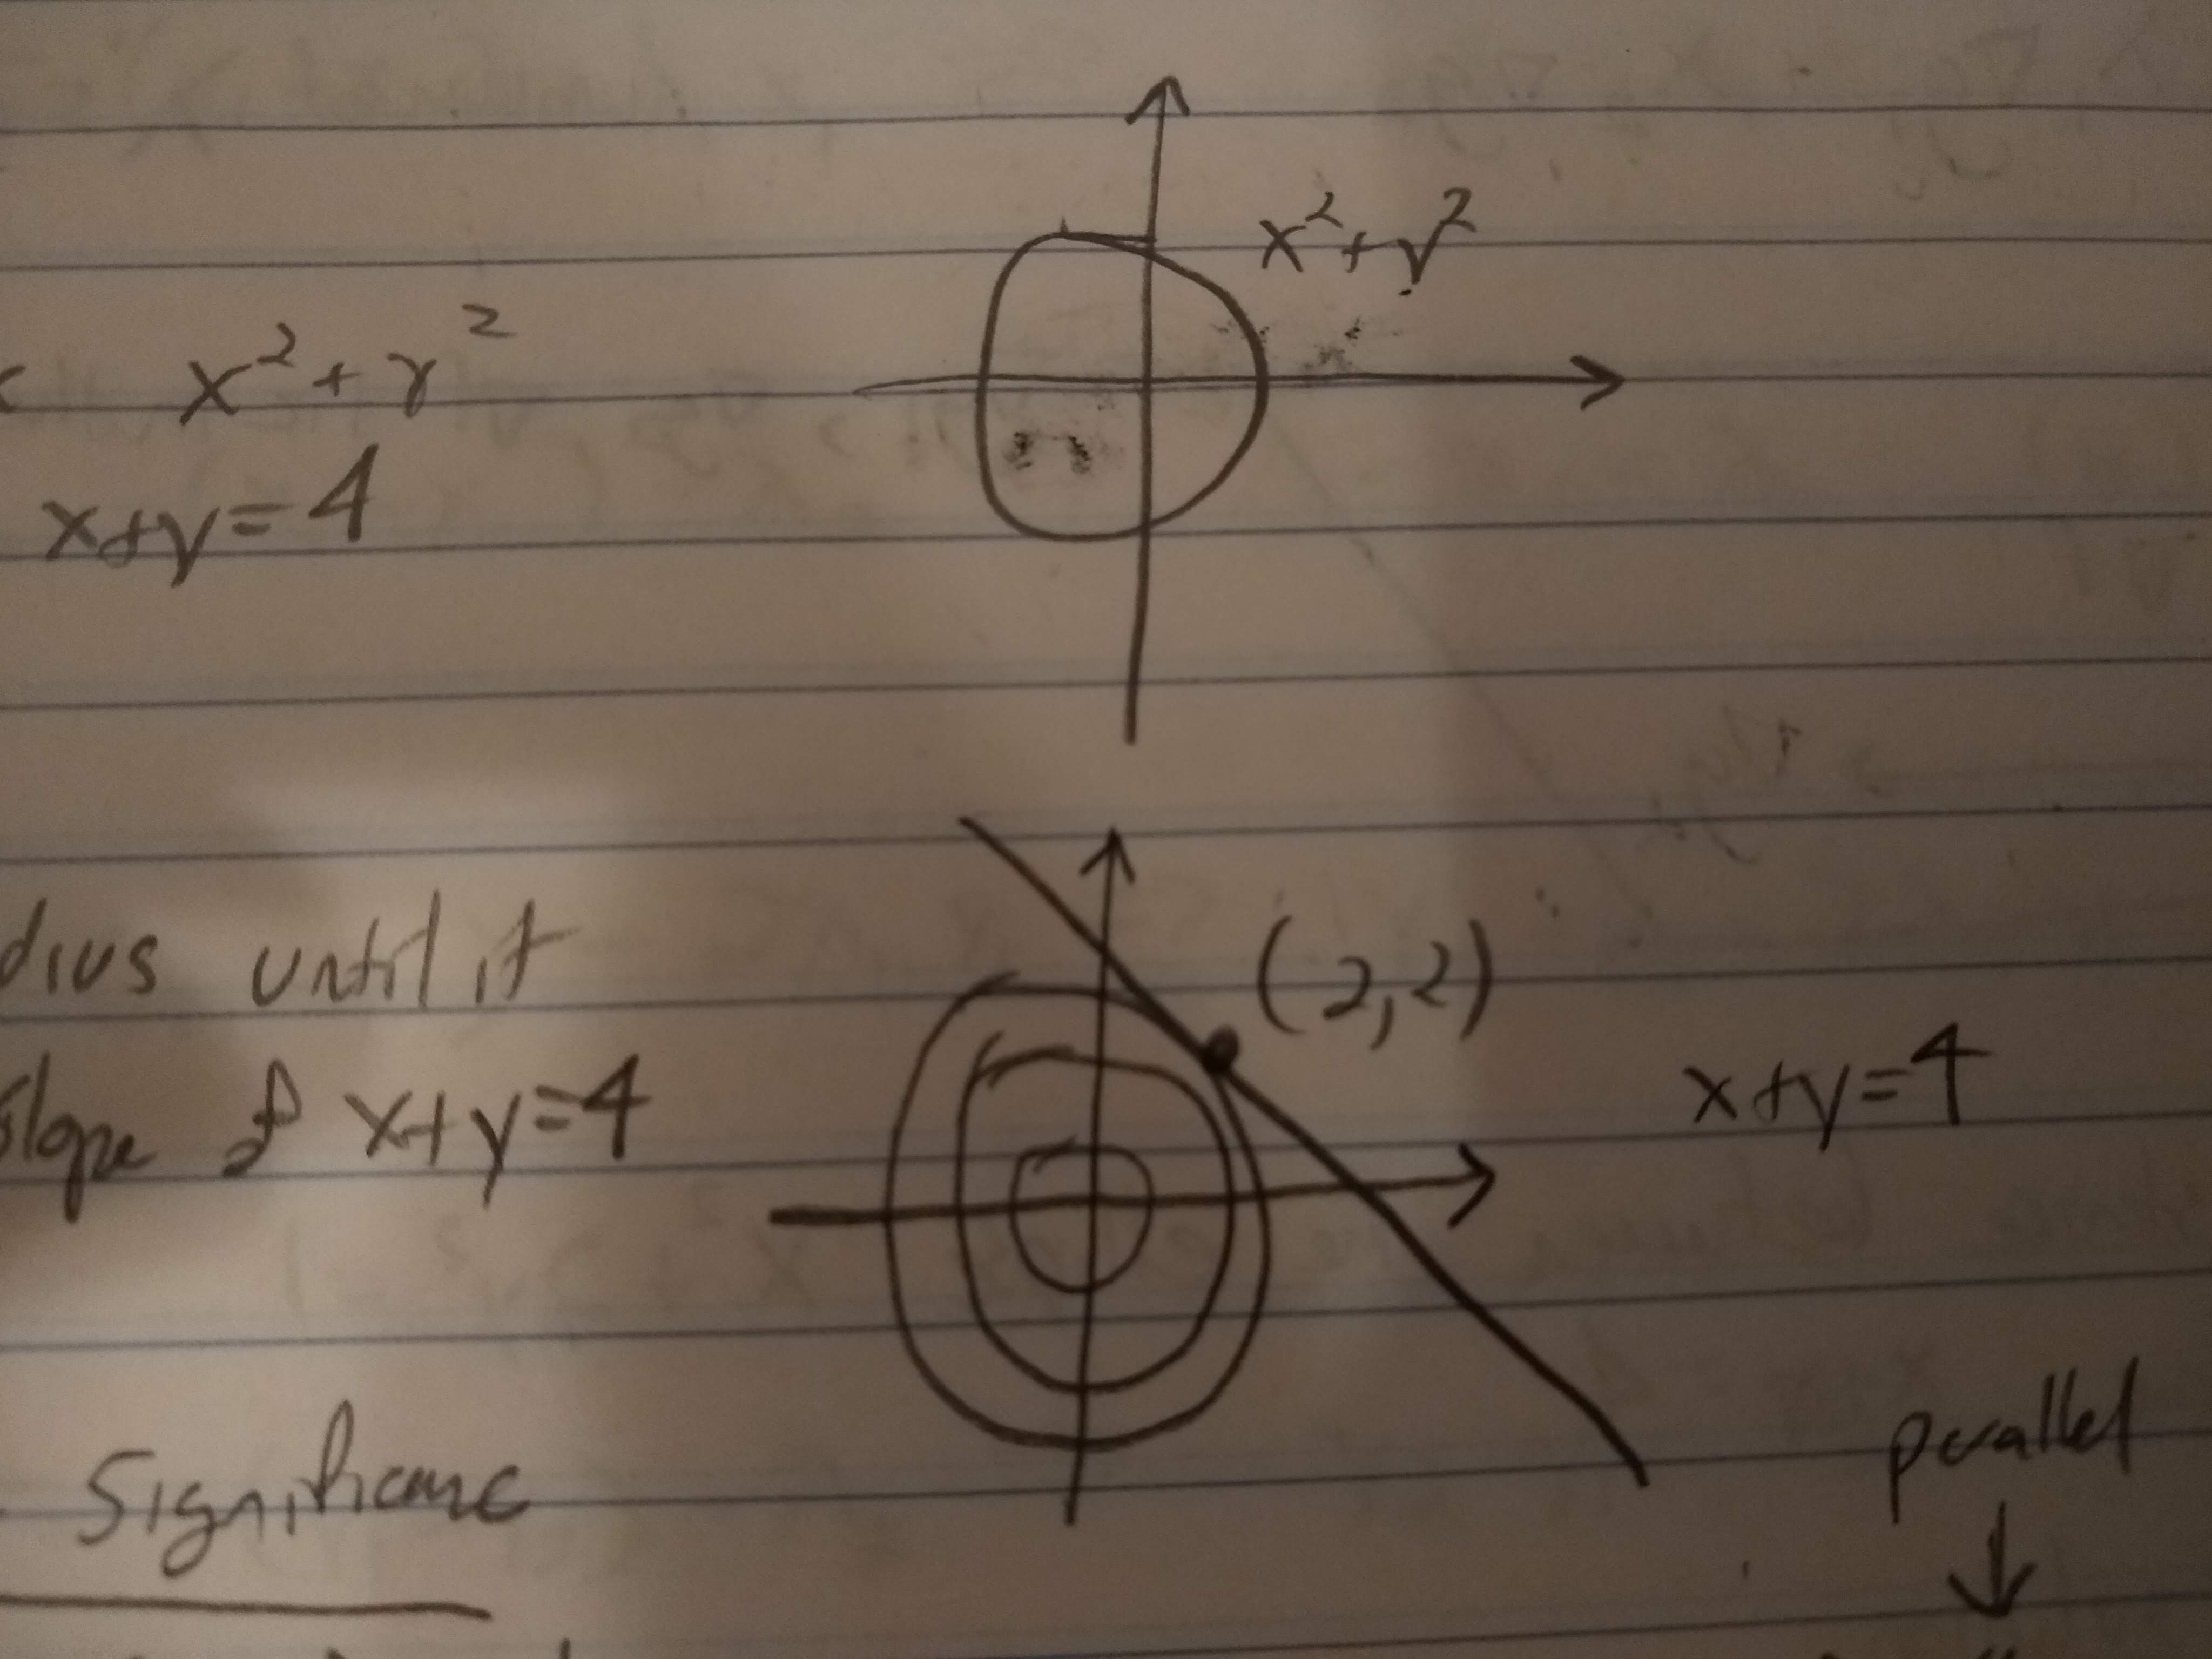
\includegraphics[width=6cm,height=4cm]{./resources/lagrangian_prelude.jpg}
\caption{\label{fig:org117831d}Prelude Drawgin}
\end{figure}

\subsubsection{Geometric Significance}
\label{sec:orgeffea85}

A \((x, y) = (2, 2)\) where MAX occurs: \(\nabla f // \nabla g\)

\(f(x, y) = x^2 + y^2; \ \nabla f = (2x, 2y)\)

\(g(x, y) = x + y - 4 = 0;\)

\$ \(\nabla\) g = (1, 1)\$

\begin{equation}
\begin{split}
\nabla f = & \lambda \nabla g & \ \text{another way of saying parallel}\\
= & (2x, 2y) = (4, 4)
\end{split}
\end{equation}

\subsection{Lagrange Multipliers}
\label{sec:orgbe92aeb}
with Several inequality constraints

\begin{quote}
Karush Kahn Tucker
\end{quote}

\uline{Goal}: Get the background to understand Lagrange Duality

\uline{Idea}: Find a MAX or MIN of \(f(x_1, x_2, y_1, y_2)\) subject to 3 requirements
(constraints)

\begin{equation}
\begin{split}
g_1(x_1, x_2, y_1, y_2) = & 0\\
g_2(x_1, x_2, y_1, y_2) = & 0\\
\end{split}
\end{equation}



\begin{itemize}
\item \(f (\cdot)\) can have any number of variables
\item can be subject to any constraint
\end{itemize}

Famous application in ML: SNMF (Semi-nonnegative Matrix Factorization)

\subsubsection{Geometric Condition}
\label{sec:org5e44f86}

The gradient of \(f\) is a \uline{Linear Combination} of the gradients of \(g_1\) and
\(g_2\). The number of \(\lambda =\) number of constraints.

$$
\nabla f = \lambda_1 \nabla g_1 + \lambda_2 \nabla g_2
$$

\begin{figure}[htbp]
\centering
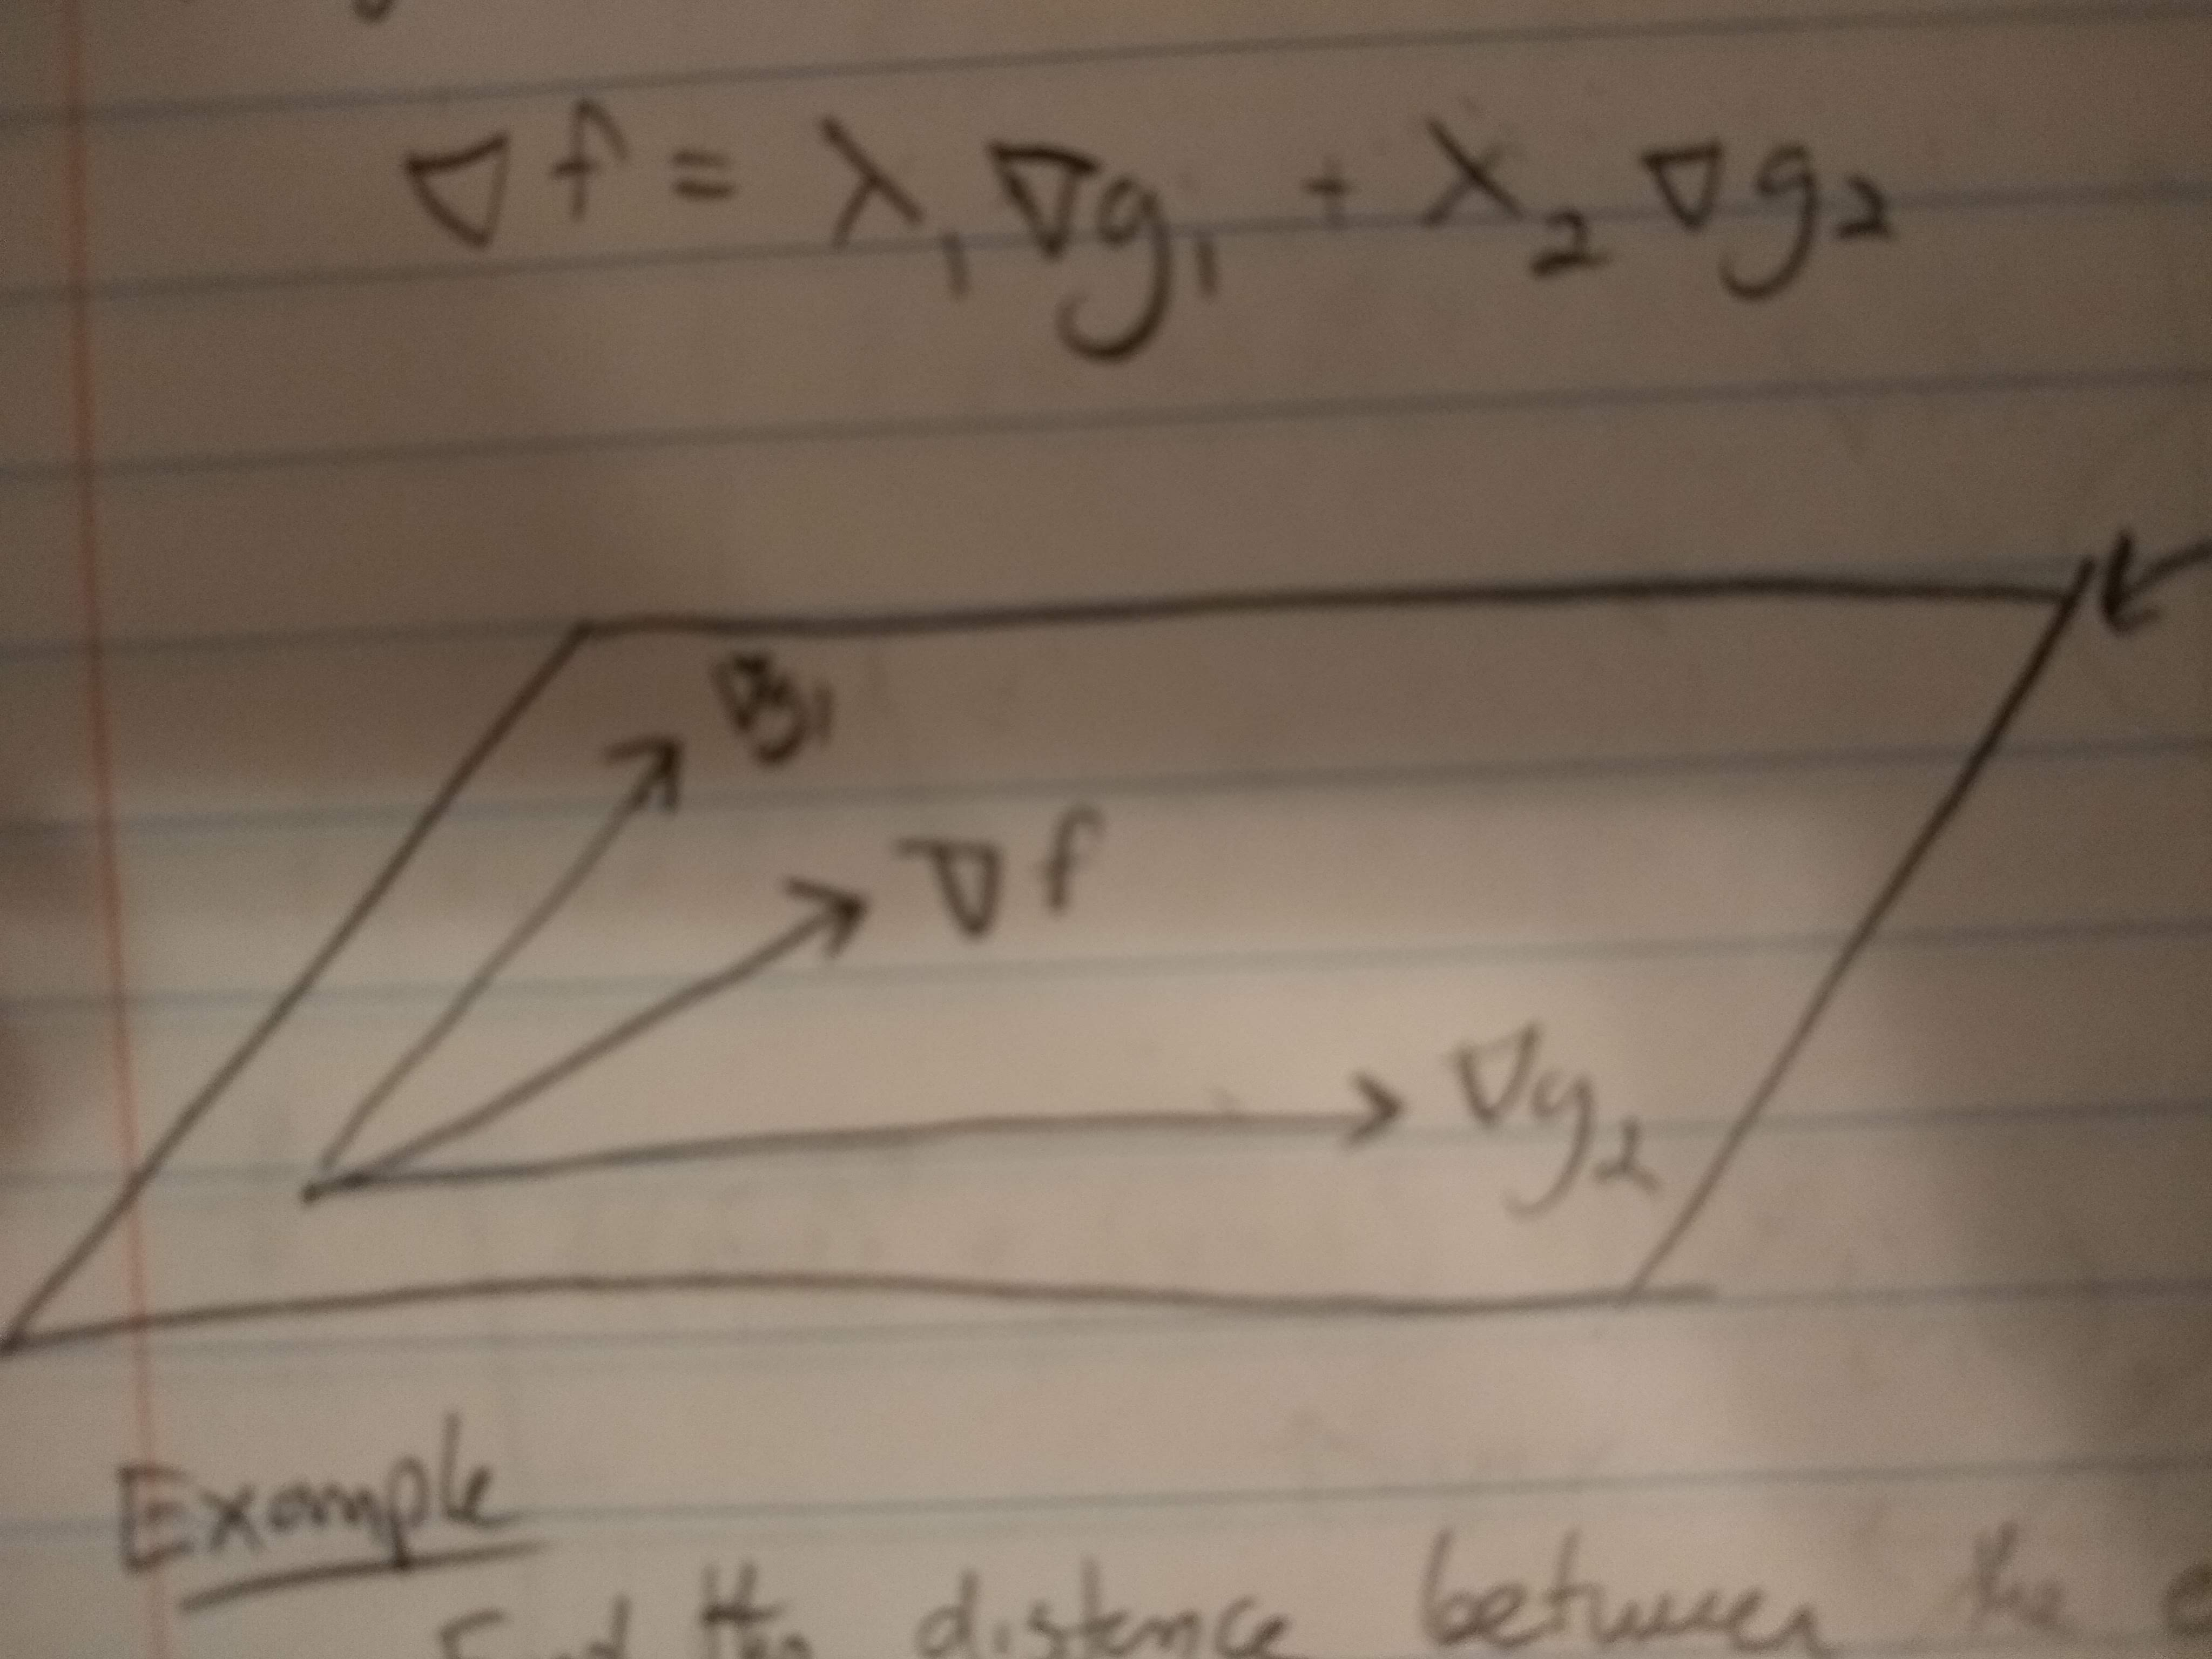
\includegraphics[width=5cm,height=3cm]{./resources/lagrangian_planes.jpg}
\caption{\label{fig:orgf5c6cea}Hyperplane of Gradients and vector function}
\end{figure}

\$ \(\nabla\) g\textsubscript{1}, $\backslash$ \(\nabla\) g\textsubscript{2}, $\backslash$ \(\nabla\) f\$ lie in the \uline{same} plane.

\begin{enumerate}
\item Example
\label{sec:org583598c}

Find the distance between the ellipse \(x^2 + 2 y^2 = 1\) and the line \(x + y =
4\).

\uline{Main Idea of the Solution}

Let \((x_1, y_1)\) be any point on the ellipse and \((x_2, y_2)\) be on any point on
the line.

$$
min \ d^2 = (x_1 - x_2)^2 + (y_1 - y_2)^2
$$

\^{}\textsuperscript{f}

subject to

$$x_1^2 + 2y_!^2 = 1, \ x_2 + y_2 = 4$$

\uline{Setting}: To find MIN of \(f\), subject to \(g_1 = 0\) and \(g_2 = 0\) where

$$
g_1 = x_1^2 + 2y_1^2 - 1, \ g_2 = x_2 + y_2 - 4
$$


\uline{Strategy}: Let \(F = f - \lambda_1 g_1 - \lambda_2 g_2\) where F is the
\textbf{Lagrangian}

\begin{equation}
\begin{split}
\nabla F = & \nabla f - \lambda_1 \nabla g_1 - \lambda_2 \nabla g_2\\
0 = & \nabla f - \lambda_1 \nabla g_1 - \lambda_2 \nabla g_2\\
\nabla f = & \lambda_1 \nabla g_1 + \lambda_2 \nabla g_2
\end{split}
\end{equation}

Let

$$
F = \frac{1}{2} [(x_1 - x_2)^2 + (y_1 - y_2)^2] - \frac{\lambda_1}{2}(x_1^2 + 2
y_1^2 - 1) - \lambda_2 (x_2 + y_2 - 4)
$$

Take all partial derivatives. set \(\nabla F = \vec 0\)

\begin{subequations}
\label{first:two}
\begin{align}
\frac{\partial F}{\partial x_1} = (x_1 - x_2)  - \lambda_1 x_1 \to & \ x_1 - x_2 = \lambda_1 x_1\\
\frac{\partial F}{\partial y_1} = (y_1 - y_2) - 2 \lambda_1 y_1 \to & \ y_1 - y_2 = 2 \lambda_1 y_1\\
\frac{\partial F}{\partial x_2} = -(x_1 - x_2) - \lambda_2 \to & \ x_2 - x_1 = \lambda_2\\
\frac{\partial F}{\partial y_2} = - (y_1 - y_2) - 2 \lambda_2 \to & \ y_2 - y_1 = \lambda_2\\
\end{align}
\end{subequations}

$$
\lambda_2 = - \lambda_1 x_1, \ \lambda_2 = -2 \lambda_1 y_1
$$

(1)(3), (2)(4)

\begin{quote}
\(\lambda_1 \neq 0\). If \(\lambda_1 = 0\), then \(x_1 = x_2\) which means the ellipse
and the line touch (which they don't). There is no common intersection point.
\end{quote}

From (1), \(\lambda \neq 0\), therefore \(x_1 = 2 y_1\)


Since \(x_1^2 + 2 y_1^2 = 1\) and \((x_1, y_1)\) is in the first quadrant, so using
\(x_1 = 2 y_1\).

$$
(x_1, y_1) = (\frac{2}{\sqrt 6}, \ \frac{1}{\sqrt 6})
$$

Using (3)(4) to solve for \((x_2, y_2)\).

Once we have \((x_1, y_1), \ (x_2, y_2)\), compute \(s^2 = (x_1 - x_2)^2 + (y_1 -
y_2)^2\). The distance between the ellipse and the line is the value of \(d\).

$$
F(x_1, x_2, y_1, y_2) = f - \lambda_1 g_1 - \lambda_2 g_2
$$

Then set \(\nabla F = \vec 0\).

What are Lagrangian Multipliers doing? It turns a constrained optimization
problem into an UNCONSTRAINED optimization problem.

Does this method work in general?

\begin{figure}[htbp]
\centering
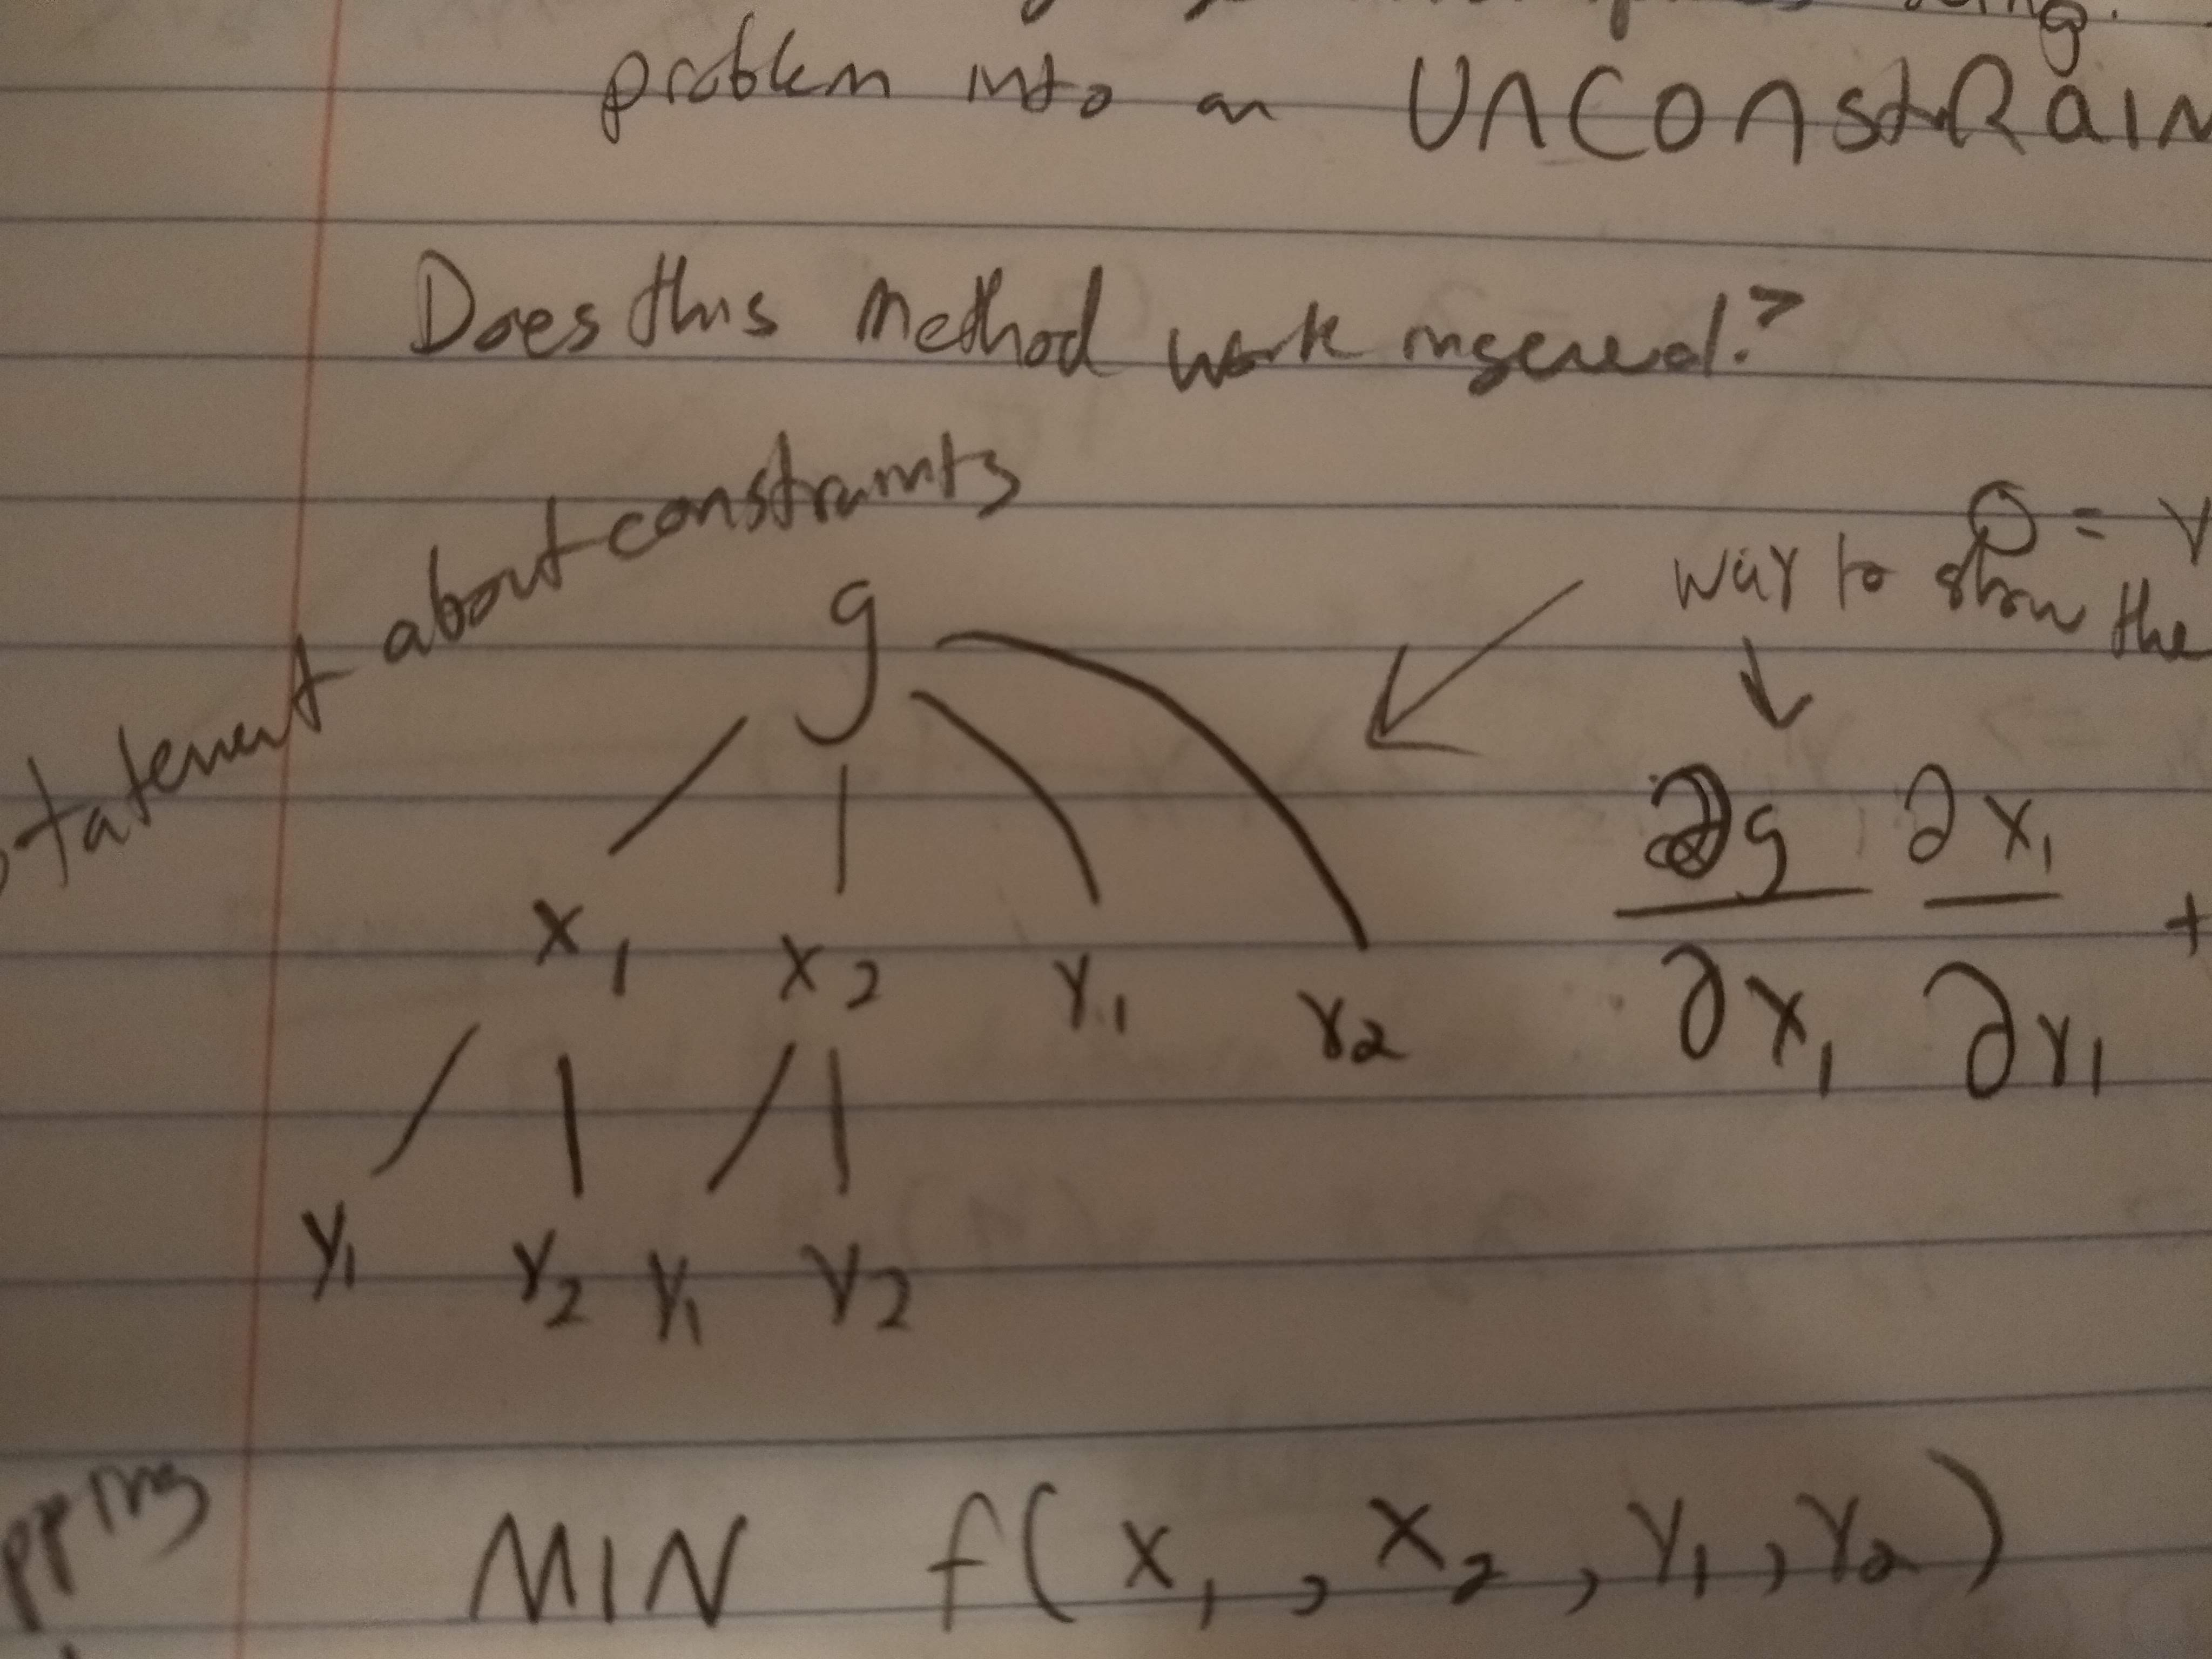
\includegraphics[width=6cm,height=4cm]{./resources/chain_rule.jpg}
\caption{\label{fig:org66344c6}Breaking Down the Chain Rule}
\end{figure}

\(\frac{\partial g}{\partial x_1} \frac{\partial x_2}{\partial y_1} + \frac{\partial g}{\partial x_2} \frac{\partial x_2}{\partial y_1} + \frac{\partial g}{\partial y_1} = 0\)

\(C^1\) mapping from \(h_1 \to h_2\).

\(\exists h_1, \ h_2\) such that

$$
x_1 = h_1 (y_1, y_2), \ x_2 = h_2 (y_1, y_2)
$$

Some function exists of \(y_1, y_2\) called \(h_1, h_2\). This comes from the \textbf{constraints}.

This is due to the \textbf{Implicit Function Theorem}. We never use \(f\) to determine
\(h_1, h_2\) which means we can have \(f\) be \emph{anything}. It is important because we
know f is a function \(y_1\) and \(y_2\) only, which means we only have to take
derivatives of \(y_1\) and \(y_2\).
\end{enumerate}

\subsubsection{Explain Why Lagrange Multipliers Work}
\label{sec:org168311e}

How do we know \(\lambda_1, \ \lambda_2\) exist?

Optimization Problem: MIN \(f (x_1, x_2, y_1, y_2)\) subject to constraints

\begin{equation}
\begin{split}
g_1 (x_1, x_2, y_1, y_2) = & 0\\
g_2 (x_1, x_2, y_1, y_2) = & 0\\
\end{split}
\end{equation}

\begin{quote}
\(h_1\) and \(h_2\) are smooth as \(g_1\) and \(g_2\).
\end{quote}

\(\exists \ h_1, \ h_2\) such that \(x_1 = h_1 (y_1, y_2), \ x_2 = h_2 (y_1, y_2)\)


\begin{equation}
\begin{split}
\to & g_1 (h_1(y_1, y_2), h_2 (y_1, y_2), y_1, y_2) = 0\\
\to & g_2 (h_1(y_1, y_2), h_2 (y_1, y_2), y_1, y_2) = 0\\
\end{split}
\end{equation}

Take partial derivatives with respect to \(y_1\)
\begin{itemize}
\item from \(g_1\)
\end{itemize}

\(\frac{\partial g_1}{\partial y_1} + \frac{\partial h_1}{\partial y_1}
\frac{\partial g_1}{\partial x_1} + \frac{\partial h_2}{\partial y_1} \frac{\partial g_1}{\partial x_2} = 0\)

\begin{itemize}
\item from \(g_2\), we get
\end{itemize}

\(\frac{\partial g_2}{\partial y_1} + \frac{\partial h_1}{\partial y_1}\frac{\partial g_2}{\partial x_1} + \frac{\partial h_2}{\partial y_1} \frac{\partial g_2}{\partial x_2} = 0\)

\begin{itemize}
\item to minimize \(f(x_1, x_2, y_1, y_2)\)
\end{itemize}


\(\frac{\partial f}{\partial y_1} + \frac{\partial f}{\partial x_1}\frac{\partial h_1}{\partial y_1} + \frac{\partial f}{\partial x_2} \frac{\partial h_2}{\partial y_1} = 0\)

\begin{equation}
\begin{split}
\begin{bmatrix}
\frac{\partial f}{\partial y_1} & \frac{\partial f}{\partial x_1} & \frac{\partial f}{\partial x_2}\\
\frac{\partial g_1}{\partial y_1} & \frac{\partial g_1}{\partial x_1} & \frac{\partial g_1}{\partial x_2}\\
\frac{\partial g_2}{\partial y_1} & \frac{\partial g_2}{\partial x_1} & \frac{\partial g_2}{\partial x_2}\\
\end{bmatrix} \begin{bmatrix}
1\\ \frac{\partial h_1}{\partial y_1}\\ \frac{\partial h_2}{\partial y_1}
\end{bmatrix} = \begin{bmatrix}
0\\ 0\\ 0\\
\end{bmatrix} & \text{(*)}
\end{split}
\end{equation}

Let A be the \(3 \times 3\) matrix on the left side. Suppose \(A^{-1}\) exists, then
multiplying both side by \(A^{-1}\).

\begin{equation}
\begin{split}
\begin{bmatrix}
1\\ \frac{\partial h_1}{\partial y_1}\\ \frac{\partial h_2}{\partial y_1}
\end{bmatrix} = \begin{bmatrix}
0\\ 0\\ 0
\end{bmatrix}
\end{split}
\end{equation}

\textbf{Not True} thus \(A^{-1}\) cannot exist.

If \(\nabla g_1\) and \(\nabla g_2\) are linearly independent, then the top row is a
linear combination of \(\nabla g_1\) and \(\nabla g_2\). (Otherwise the matrix would
be invertible).

As long as your constraints are linearly independent, then the function is a
linear combo of the gradients of the constraints.


\subsection{Application}
\label{sec:org7558d0b}

Non-Negative Matrix Factorization

\(B \geq 0\) denotes a matrix with non-negative entries.

We use the Frobenius Norm (Hilbert-Schmidt Norm)

$$
\|B\|_F^2 = \Sigma_j \Sigma_k |B(j, k)^2|
$$

Given an \(m \times n\) non-negative matrix A, NMF is defined as

\begin{equation}
\begin{split}
\underset{x \in R^{m \times r, \ Y \in R^{r \times m}}}{\|A - XY\|_F^2} & \text{s.t.} \ x \geq 0, \ Y \geq 0
\end{split}
\end{equation}

Where r is the parameter that controls the size of factors X, Y.

Let A be a \(1000 \times 1000\) image. Each pixel is a nonnegative number from \(0
\to 255\). We \uline{hope} to discover the structure of A by writing \(A = X_Y\) where X
has 60 columns.

The column vectors \(a_1, a_2, ..., a_{1000} \in R^{1000}\) belong to a
60-dimensional subspace. A has 1 million entries. X has 60,000 entries and Y has
60,000 entries.

Since A is a non-negative matrix, it makes sense that at least one of X and Y is
non-negative.

$$
a_1, a_2, a_3, ... \in Span\{x_1, x_2, ..., x_{60}\}, \ \text{each} \ \ x_j \in R^{1000}
$$

\(a_5 = c_1 x_1 + c_2 x_2 + ... + c_{60} x_{60}\)

This problem can be formulated as the following:

\begin{equation}
\begin{split}
\underset{X,U \in R^{m \times r, \ Y,V \in R^{r \times m}}}{\|A - XY\|_F^2} & \text{s.t.} U = X, \ V = Y, \ \ x \geq 0, \ Y \geq 0
\end{split}
\end{equation}

Where we introduced artificial variables for matrices U,V.

We consider the \textbf{Augment Lagrangian} of the Problem.

\begin{quote}
``Augmented'' means to increase in mathematical terms.
\end{quote}

$$
\mathcal L = \|A - XY\|_F^2 + \langle \Lambda, X - U \rangle + \langle \Phi, Y -
V \rangle + \frac{\alpha}{2} \|X - U\|_F^2 + \frac{\beta}{2} \|Y - V\|_F^2
$$


\(\|A - XY\|_F^2\): Objective Function

\(\Lambda, \ \Phi\): Lagrange Multipliers that are Matrices

\(\Lambda\) is the same size as X

\(\Phi\) is the same size as Y

\begin{quote}
Inner product of A,B = \(\langle A, B \rangle = Tr(A^T B)\)
\end{quote}

\uline{Remark}: \(\mathcal L\) is a function of entries \(X, Y, U, V\).

It is possible to compute partial derivatives such as

$$
\frac{\partial \mathcal L}{\partial x_{1,1}}, \ \frac{\partial \mathcal
L}{\partial x_{1,2}}, \ \frac{\partial \mathcal L}{\partial y_{1,1}}, \ \frac{\partial \mathcal L}{\partial y_{1,2}}
$$

\subsubsection{An Approach to NMF Using ADMM}
\label{sec:orgce33cb0}

Input: A \(m \times n\) matrix A, Target Rank R.

Alternating Direction Method of Multipliers

Output: A \(m \times r\) matrix U, an \(r \times n\) matrix V.

K = 1, \ldots{}, N

\begin{equation}
\begin{split}
X_{k + 1} = & (A Y_k^T + \alpha U_k - \Lambda_k) (Y_k Y_k^T + \alpha I)^{-1}\\
Y_{k + 1} = & (X_{k + 1}^T X_{k + 1} - \beta I)^{-1} (X_{k + 1}^T \Lambda + \beta V_k - \Phi_k)\\
\end{split}
\end{equation}

Update \(U_{k + 1}\) using \(X_{k + 1}\) and \(\Lambda_k\)

Update \(V_{k + 1}\) using \(Y_{k + 1}\) and \(\Phi_k\)

Update \(\Lambda_{k + 1}\) and \(\Phi_{k + 1}\)
\section{Lagrangian Multipliers \& Optimal Margin Classifiers (2020/05/19)}
\label{sec:org07b4661}
\subsection{Warm Up}
\label{sec:orge942742}
\begin{figure}[htbp]
\centering
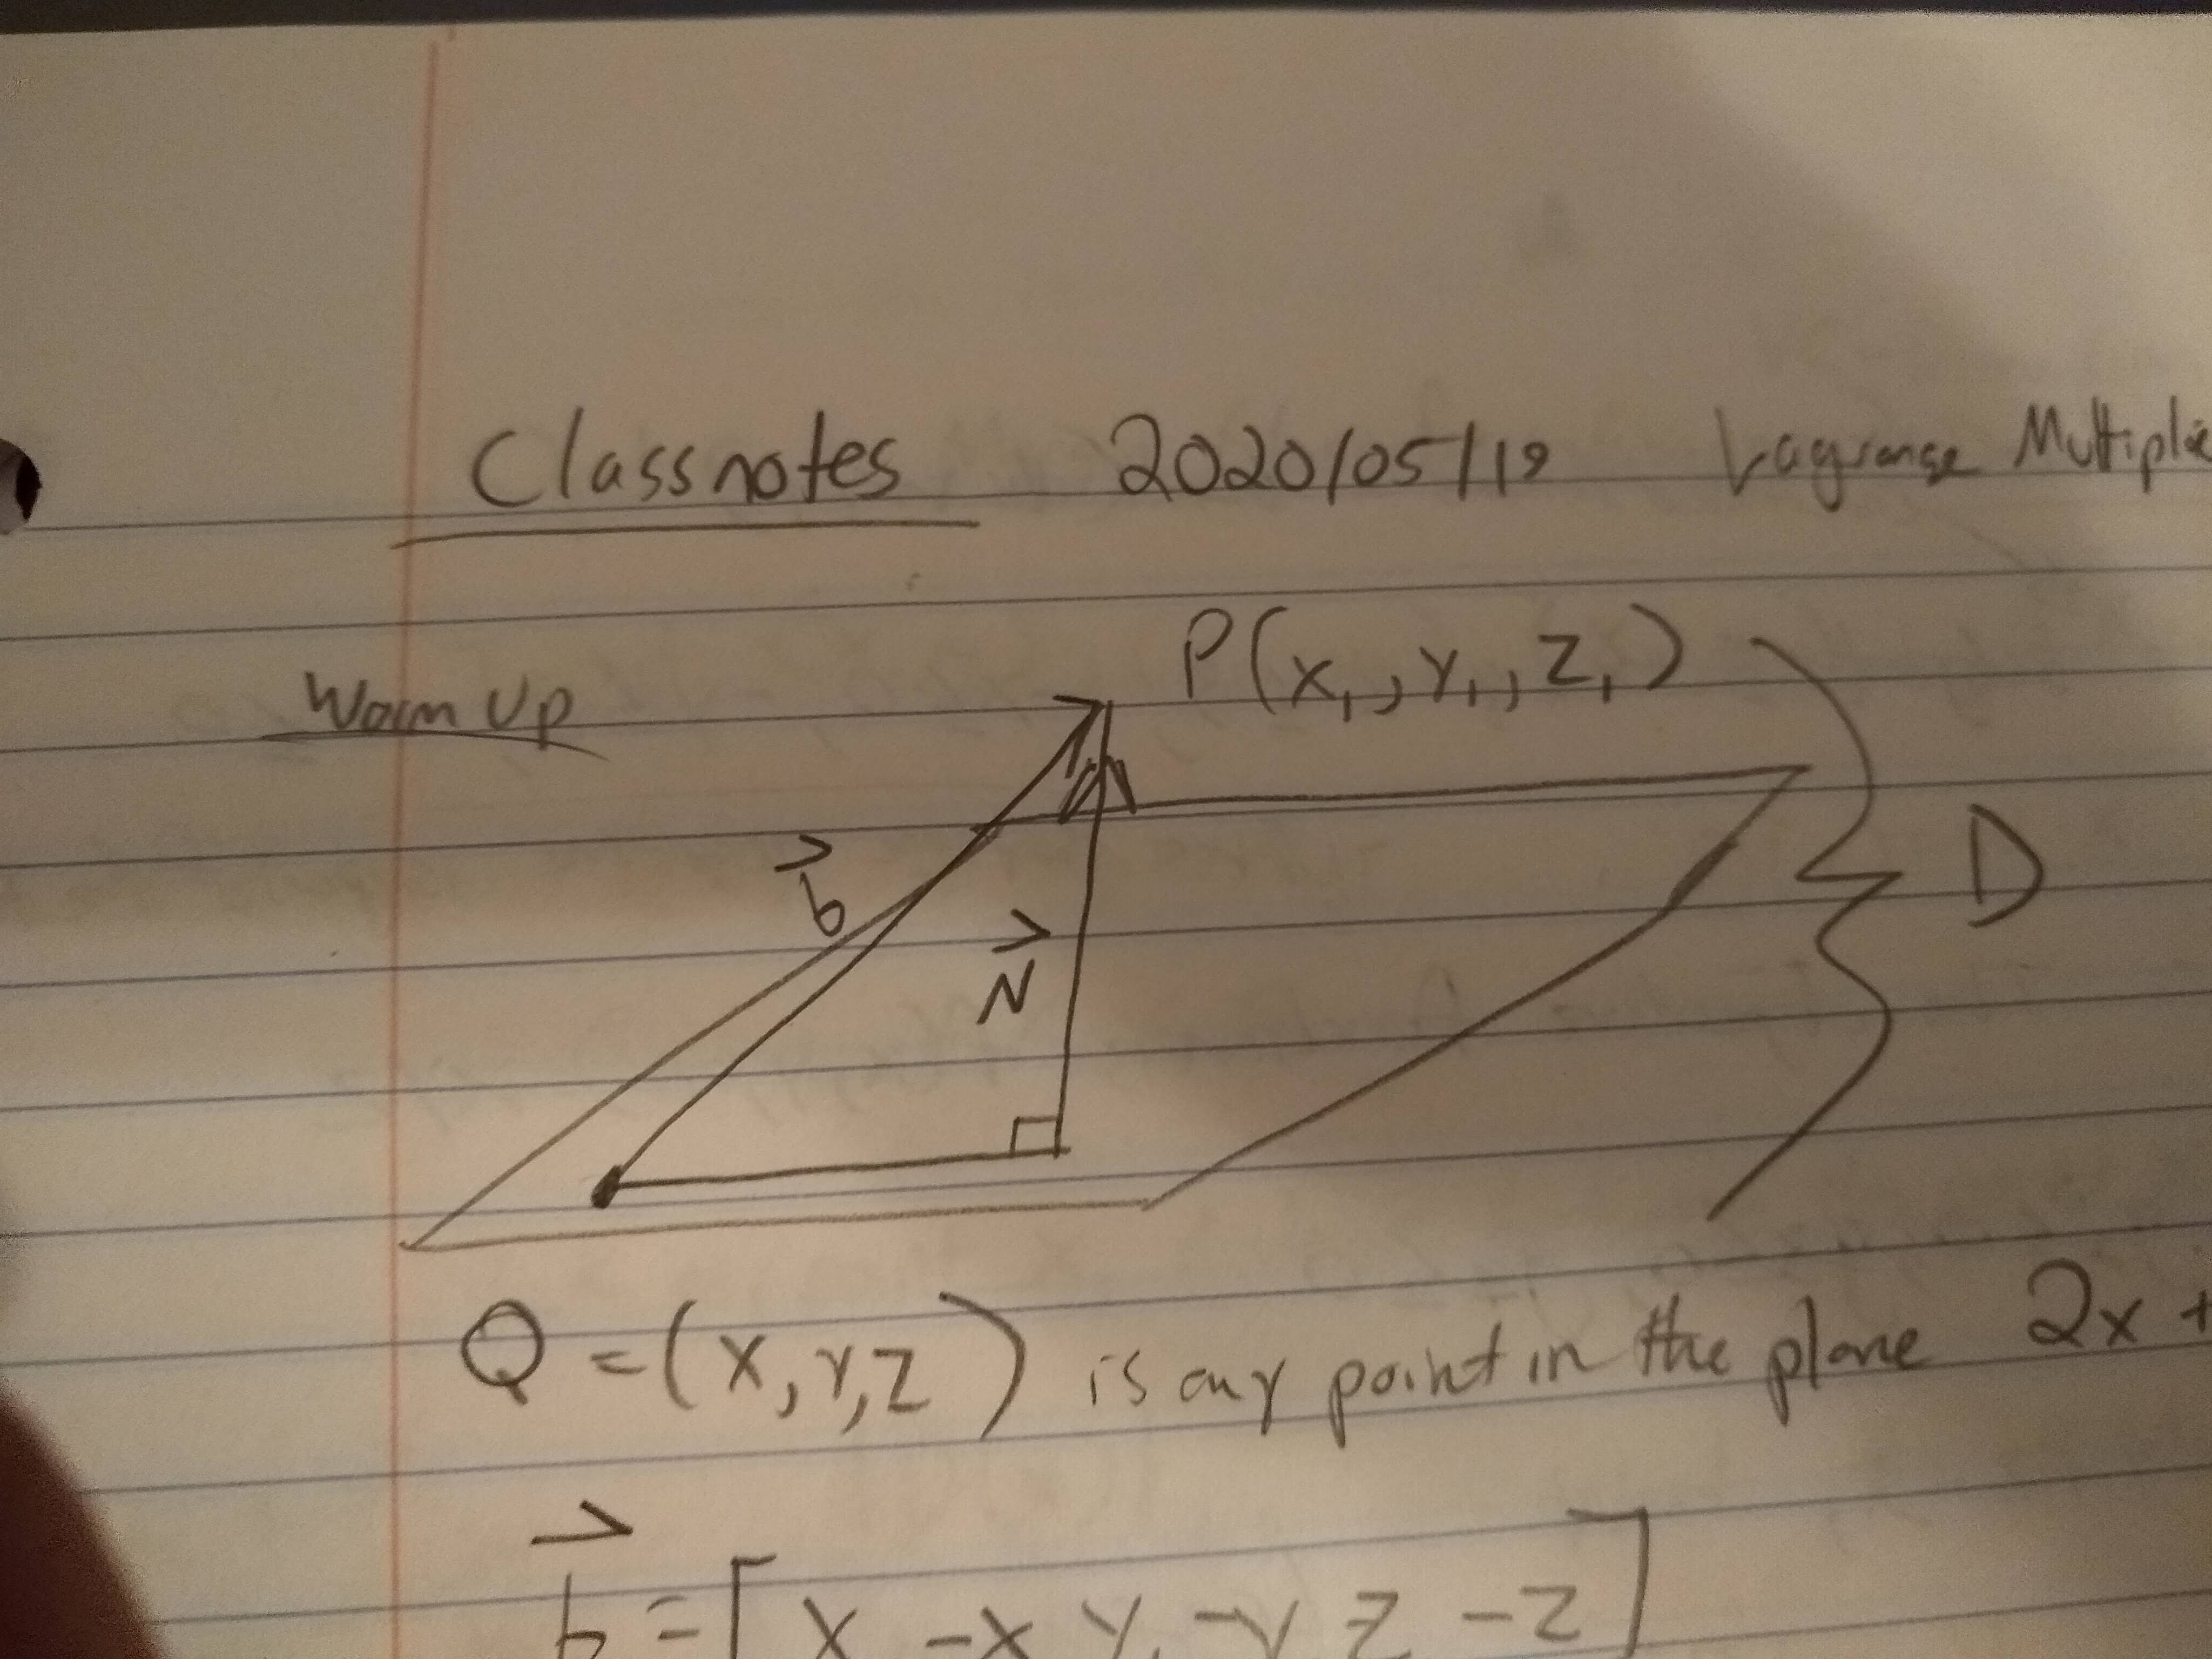
\includegraphics[width=6cm,height=4cm]{./resources/warmup_plane.jpg}
\caption{\label{fig:org6a63ea5}Warm Up Plane}
\end{figure}

\(Q = (X, Y, Z)\) is any point in the plane \(2x + 3y + 4z = 5\)

\(\vec b = [x, -x, y, -y, z, -z]\)

\begin{equation}
\begin{split}
D = & \frac{\|\vec N \cdot \vec b\|}{\|\vec N\|}, \ \vec N = [2, 3, 4]\\
= & \frac{\|2(x_1 - x) + 3(y_1 - y) + 4(z_1 - z)\|}{\|\vec N\|}\\
= & \frac{\|(2 x_1 + 3 y_1 + 4 z_1) - (2x + 3y + 4z)\|}{\|\vec N\|}\\
= & \frac{\|(2x_1 + 3 y_1 + 4 z_1) - 5\|}{\|\vec N\|}
\end{split}
\end{equation}

Input: \((\vec X_1, Y_1),(\vec X_2, Y_2),(\vec X_3, Y_3)\)

where \(\begin{cases} Y_k = 1 & \vec X_k \in A\\ Y_k = -1 & \vec X_k \in B \end{cases}\)

\(\begin{cases} \vec X \in A & D(\vec X) > 0\\ \vec X \in B & D(\vec X) \leq 0 \end{cases}\)

\(D(\vec X) = \vec W \cdot \vec X\)

\(D(X)\): The decision function

\begin{figure}[htbp]
\centering
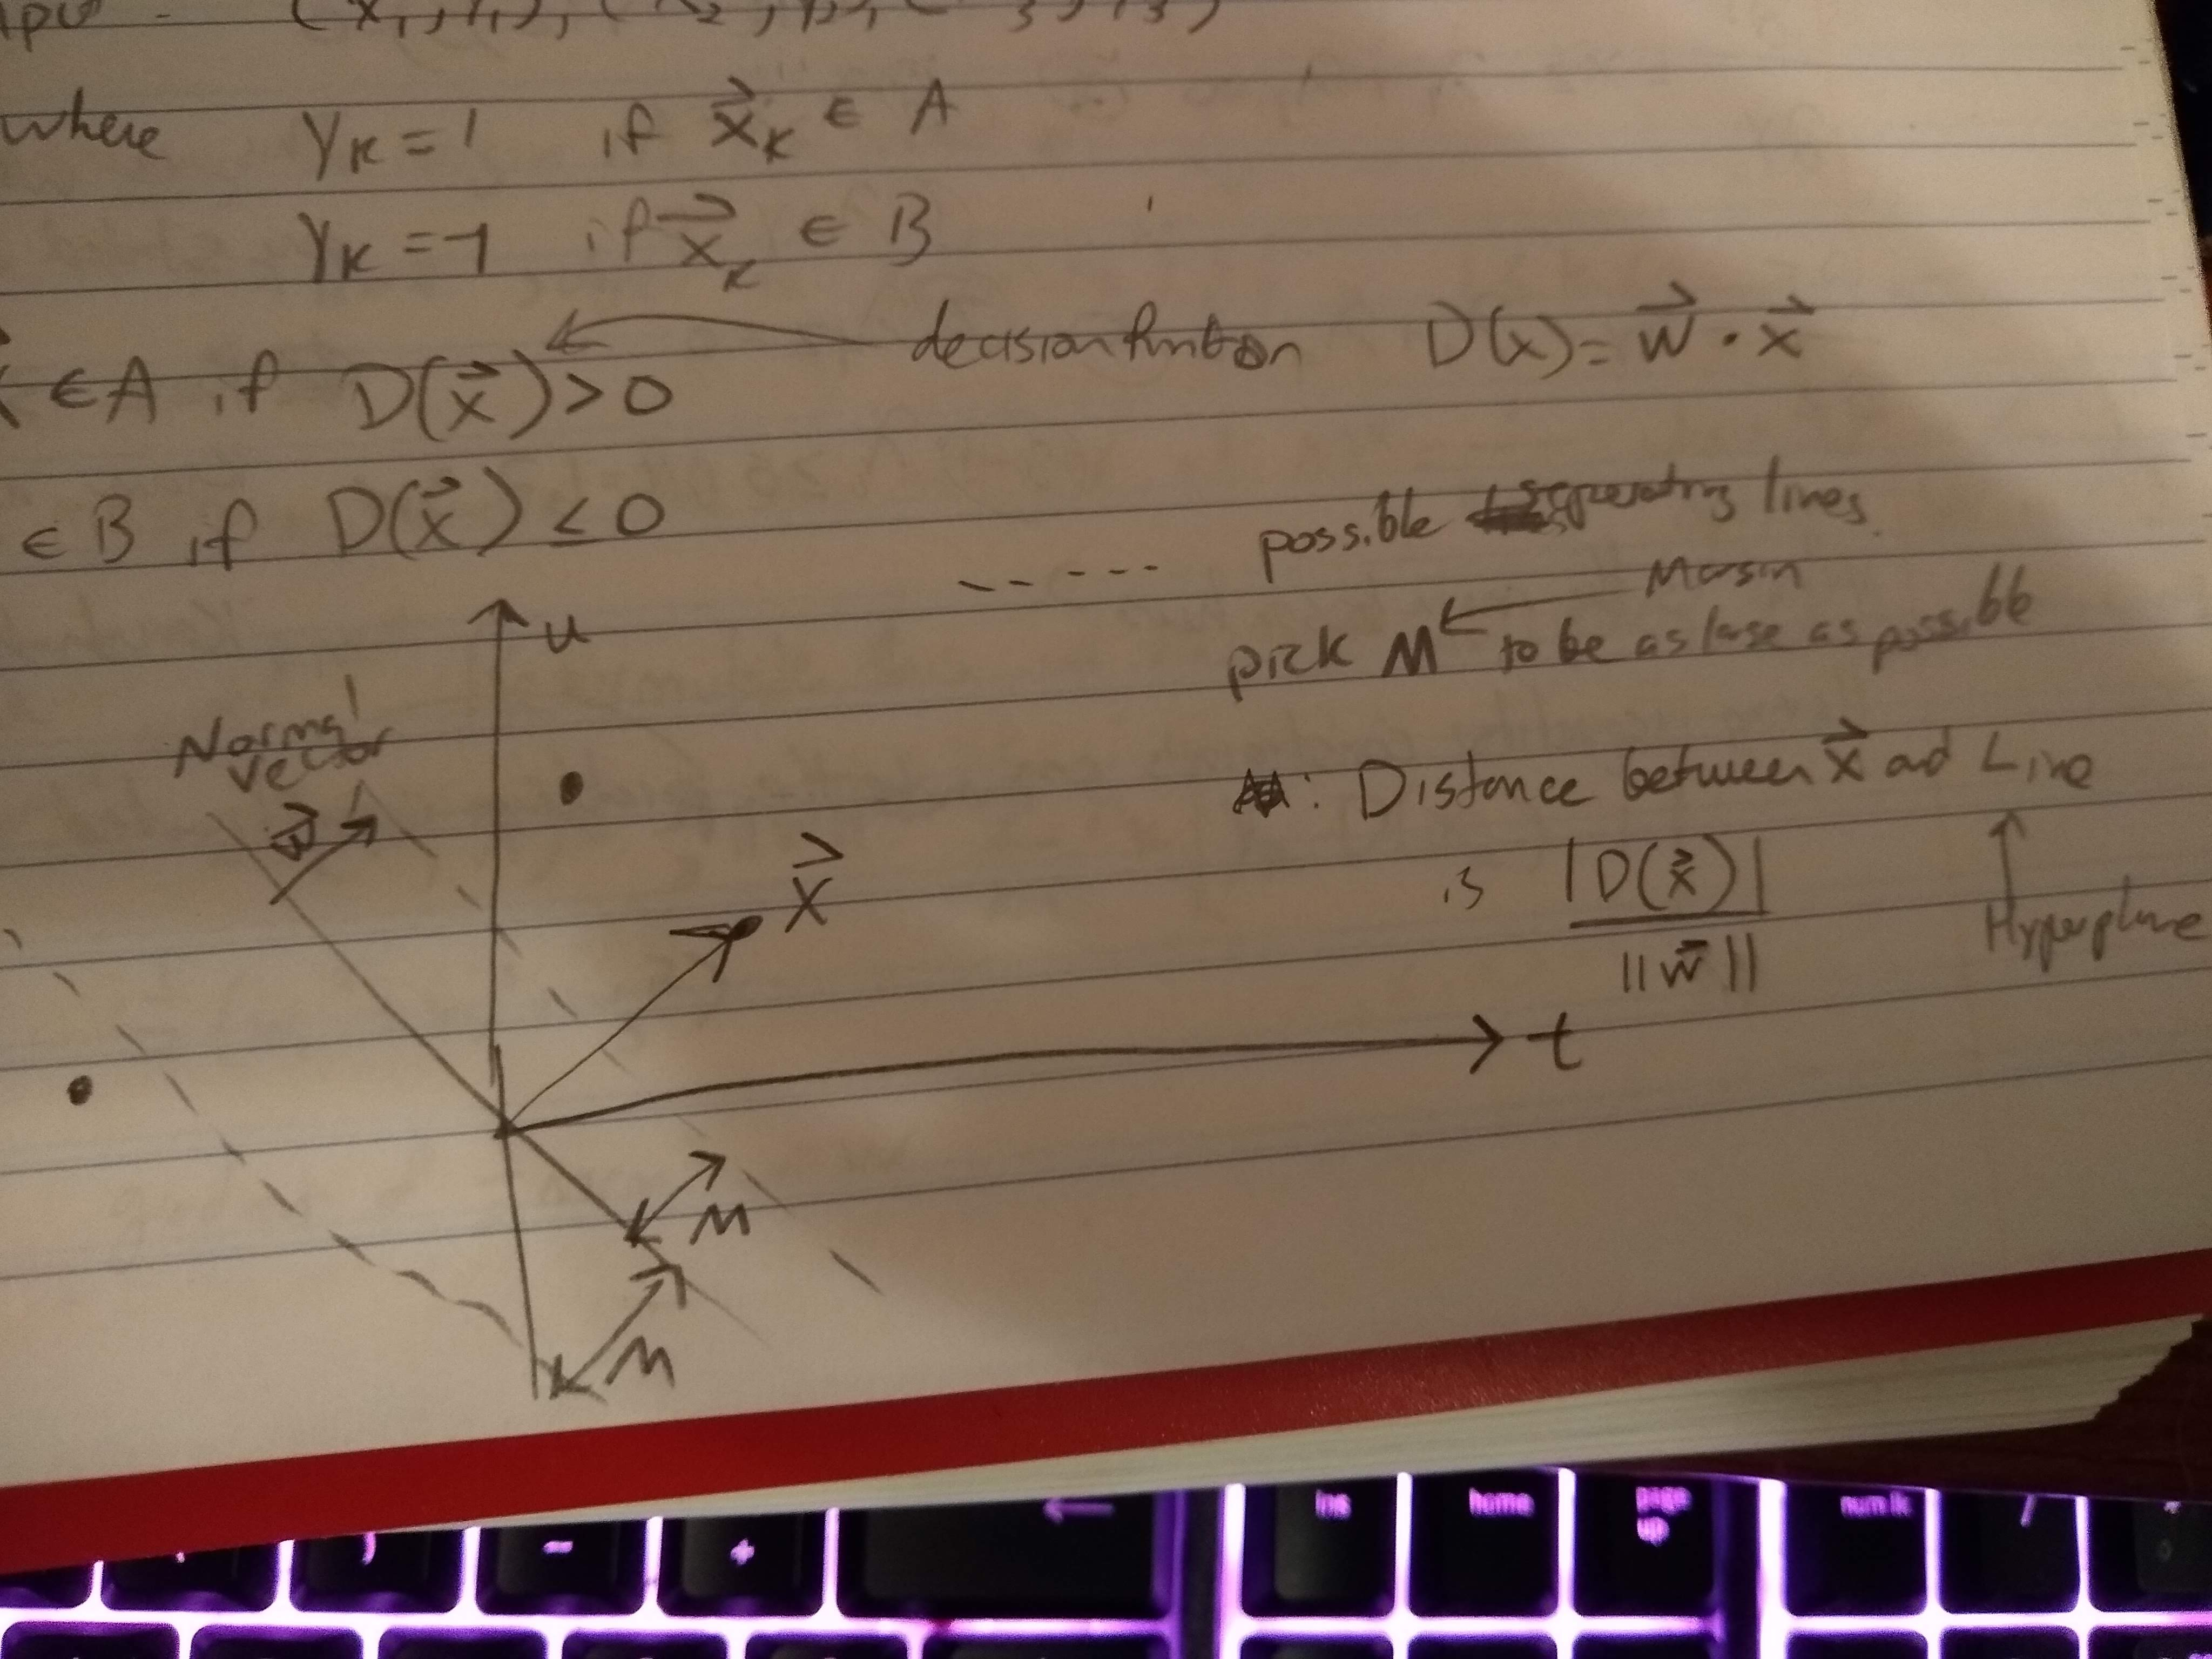
\includegraphics[width=6cm,height=4cm]{./resources/warmup2.jpg}
\caption{\label{fig:org779c800}Warmup (cont)}
\end{figure}

\subsection{Lagrange Multipliers}
\label{sec:orgf8a7d78}

\uline{Example}

Minimize xyz subject to \(x + y + z \leq 3, \ -x \leq 0, \ -y \leq 0, -z \leq 0\)

Outline of Main Idea: The objective function is \(f(x, y, z) = xyz\)

$$
g_1 \leq 0, \ g_2 \leq 0, g_3 \leq 0, g_4 \leq 0
$$

\textbf{Constraints}

\begin{equation}
\begin{split}
g_1 (x, y, z) = & x + y + z - 3\\
g_2 (x, y, z) = & -x\\
g_3 (x, y, z) = & -y\\
g_4 (x, y, z) = & -z\\
\end{split}
\end{equation}

\textbf{Lagrangian}

$$
F = f - \lambda_1 g_1 \lambda_2 g_2 - \lambda_3 g_3 - \lambda_4 g_4
$$

$$
F(x,y,z) = xyz = \lambda_1 (x + y + z - 3) + \lambda_2 x + \lambda_3 y +
\lambda_4 z
$$

\uline{Take all partial derivatives and set to 0}

\begin{equation}
\begin{split}
\frac{\partial F}{\partial x} = & yz - \lambda_1 + \lambda_2 = 0\\
\frac{\partial F}{\partial y} = & xz - \lambda_1 + \lambda_3 = 0\\
\frac{\partial F}{\partial z} = & yx - \lambda_1 + \lambda_4 = 0\\
\end{split}
\end{equation}

The above constraints are know as the KKT condition. (Karush-Kuhn-Tucker)

\textbf{More Constraints}

The following constraints are derived from the Complementary Selectness Condition

\begin{equation}
\begin{split}
\lambda_1(x + y + z - 3) = & 0\\
\lambda_2 X = & 0\\
\lambda_3 Y = & 0\\
\lambda_4 Z = & 0\\
\lambda_i \geq & 0, \ i = 1,2,3,4
\end{split}
\end{equation}

This is \uline{why} the inequalities are stated as negative.

What is the main lesson here?

Having inequality constraints can make the problem complicated.

\begin{quote}
No implicit Function theorem is used to prove Lagrangian Multipliers with
inequalities because it doesn't apply. The proof for why Lagrangian Multipliers
work for inequality constraints is not present here.
\end{quote}
\subsection{Optimal Margin Classifiers (Vapnik)}
\label{sec:orgfeffbb2}


Input: \((\vec X_1, Y_1),(\vec X_2, Y_2),(\vec X_3, Y_3)\)

where \(\begin{cases} Y_k = 1 & \vec X_k \in A\\ Y_k = -1 & \vec X_k \in B \end{cases}\)

\(\begin{cases} \vec X \in A & D(\vec X) > 0\\ \vec X \in B & D(\vec X) \leq 0 \end{cases}\)

\(D(\vec X) = \vec W \cdot \vec X\)

Pick any point x, distance between the point x and the Line (Separating
Hyperplane)

\begin{quote}
A plane is the set of all points perpendicular to a normal vector.
\end{quote}

\(\frac{|D(x)|}{\|w\|}\)

Desired State:

For \(k = 1,2,...,p, \ Y_K = \{-1, 1\}\),

$$
Y_k \frac{|D(x)|}{\|w\|} \geq M
$$

\begin{quote}
\(Y_k\) assumes that we are treating distances as negative. This is just
convention and may be dropped by other texts/sources.
\end{quote}

Formulate our optimization problem:

$$
\max_{w, \|w\| = 1} M
$$

Subject to,

$$
Y_k D(X_k) \geq M, \ 1 \leq k \leq p
$$

\textbf{Insight}: Maximizing the Margin M equivalent to

$$
\min_{w} \|w\|
$$

Subject to,

$$
Y_k D(X_k) \geq 1, \ 1 \leq k \leq p \ \ \ \label{eq:2}
$$

The maximum margin M is attained at \(M^* = \frac{1}{\|W^*\|}\) where \(W^*\) is the
optimal W in \(\eqref{eq:2}\)


\textbf{Reformulate with Lagrange Multipliers}

$$
\mathcal L (w, \lambda) = \frac{1}{2} \|W\|^2 - \sum_{k = 1}^{p} \lambda_k [Y_k
D(X_k) - 1]
$$

\begin{quote}
minimize the square of norm. The gradient of \(\frac{1}{2} norm^2 = w\)
\end{quote}

In \(\mathcal R^2\), suppose \(X_k = (t_k, u_k)\), then

$$
D(X_k) = D(t_k, u_k) = w_1 t_k + w_2 u_k \to \frac{\partial D(X_k)}{\partial
w_1} = t_k
$$


$$
\frac{\partial D(X_k)}{\partial w} \equiv (\frac{\partial D(X_k)}{\partial w_1},
\frac{\prtial D(X_k)}{\partial w_2})
$$

\(\frac{\partial D(X_k)}{\partial w_2} = u_k\)


$$
\frac{\partial \mathcal{L}}{\partial W} = W - \sum_{k = 1}^{p} \lambda_k Y_k X_k
= 0 \to W = \sum_{k = 1}^{p} \lambda_k Y_k X_k
$$

But \(D(x) = W \cdot X\)

\begin{equation}
\begin{split}
D(x) = & (\sum_{k = 1}^{p} \lambda_k Y_k X_k) \cdot X \ \leftarrow X_k \cdot X = \langle X_k, X \rangle\\
= & \sum_{k = 1}^{p} \lambda_k Y_k \langle X_k, X \rangle
\end{split}
\end{equation}

Going back to the earlier example\ldots{}

\((3 x_1 + 17.2 x_2 + 19.3 X_3) \cdot X = 3 \langle x_1, x \rangle + 17.2 \langle
x_2, x \rangle + 19.3 \langle x_3, x \rangle\)

\uline{Main Insight}

The function \(D(X)\) depends on \(x_1, x_2, x_3\) only through \(\langle x_1, x \rangle, \langle x_2, x \rangle, \langle x_3, x \rangle\)

We don't care about the values in \(x_1\), only the inner product of \(x_1\) and x.

\begin{quote}
\textbf{Engineering Principles}

\begin{itemize}
\item All numbers = 5
\item All functions are continuous
\item All continuous functions are polynomials
\item All polynomials are Linear
\end{itemize}
\end{quote}

Why do we assume the decision function is a linear function? Now, \(D(X)\) depends
on \(x_1, x_2, x_3\) through the inner products of X, So we pick a function \(f(X)\)
that \uline{depends only on the inner products} with x: \(\langle x_1, x \rangle, ..., \langle x_p, x \rangle\)

\begin{quote}
Don't forget the inner product is symmetric. \(\langle\) a, b \(\rangle\) = \(\langle\) b, a \(\rangle\)
\end{quote}

\(f(\bullet) = c_z K(\bullet, x_1) + ... + c_p K(\bullet, x_p)\)

\textbf{K is a Kernel function.}

\(K (x, x_1) = \langle x, x_1 \rangle\)

\(K (x, x_1) = 1 + \langle x, x_1 \rangle\) or \(K (x, x_1) =\) a function of \(\langle x, x_1 \rangle\)

\textbf{Evaluating when p = 4}

What happens at \(x_1\) and \(x_2\)?

\begin{equation}
\begin{split}
y_1 = & f(x_1) =  c_1 K (x_1, x_1) + c_2 K (x_1, x_2) + c_3 K (x_1, x_3) + c_4 K (x_1, x_4)\\
y_2 = & f(x_2) =  c_1 K (x_2, x_1) + c_2 K (x_2, x_2) + c_3 K (x_2, x_3) + c_4 K (x_2, x_4)\\
y_3 = & f(x_3) =  c_1 K (x_3, x_1) + c_2 K (x_3, x_2) + c_3 K (x_3, x_3) + c_4 K (x_3, x_4)\\
y_4 = & f(x_4) =  c_1 K (x_4, x_1) + c_2 K (x_4, x_2) + c_3 K (x_4, x_3) + c_4 K (x_4, x_4)\\
\end{split}
\end{equation}


\(K(a,b) = (1 + \langle a, b \rangle)^4\)

\(y_1, y_2, y_3, y_4 \in \{ -1, 1\}\)

4 Linear equations in 4 Unknowns: \(c_1, c_2, c_3, c_4\)

\(K(x_j, x_k) = (1 + \langle x_j, x_k \rangle)^4\)

\(Y = Ac\) where \(A\) is \(4 \times 4\), \(A(i,j) = K(X_j, x_k)\)

We can solve for \(c_1, c_2, c_3, c_4\) and obtain the function.

\(f(\bullet) = c_z K(\bullet, x_1) + ... + c_p K(\bullet, x_p)\)

When \(\bullet\) is a new data point, we can predict whether it belongs to class A
or B. If it is close to 1, it belongs to A. If it is close to -1, it is close to B.

\subsection{Applications of ML}
\label{sec:orge0ebe0d}
\subsubsection{Handwritten Digit Review}
\label{sec:orgda689a8}

\(28 \times 28\) handwritten digits.

$$
B = [\vec y_1, ..., \vec y_{4000}], \ \vec y_j \in \mathbb R^{784}
$$

\begin{itemize}
\item 800 images of 0, first 800 columns
\item 800 images of 1, next 800 columns
\end{itemize}

and so forth.

Let \(\vec f\) be a new image of digit 2. Solve for x such that \(\vec f = B \vec
x\). \(\vec x\) is 20-sparse. Would like to only see non-zero entries at position
1601-2400 (where the twos are)

B has 784 rows, 4000 columns.

\textbf{Important}

Let \(G^{500 \times 784}\) be a Gaussian Matrix.

$$
G \vec f = G B \vec x
$$

Let \(A = GB\) and \(\vec y = G \vec f\)

$$
\vec y = A \vec x
$$

Solve for \(\vec x\) by minimizing the \$l\textsubscript{1}\$-norm.

\begin{enumerate}
\item Application
\label{sec:org0da96c8}

Each trial of an experiment consists of training the machine with samples of
digits from 2,3,4,5. The goal is to distinguish 5 from 2,3,4.

One trial consists of the following steps:
\begin{itemize}
\item Take 1000 images of 2, Randomly select 800 and set aside 200
\item Take 1000 images of 3, Randomly select 800 and set aside 200
\item Take 1000 images of 4, Randomly select 800 and set aside 200
\item Take 1000 images of 5, Randomly select 800 and set aside 200
\item Use the 3200 selected images for training

\((x_1, y_1), ... , (x_p, y_p), \ p = 3200\)

each \(y_k = 1\) if digit is 5, and \(y_k = -1\) if digits are 2, 3, 4.

$$
    f(\diamond) = c_1 K(\diamond, x_1) + ... + c_p K(\diamond, x_p)
    $$

Use the polynomial kernel suggested by Vapnik et al.

$$
    K(x_i, x_j) = (1 + \langle x_i, x_j \rangle)^4
    $$
\end{itemize}


For the 200 images of 4 set aside for testing, we want to see \(f(\diamond) \approx -1\)
For the 200 images of 5 set aside for testing, we want to see \(f(\diamond) \approx 1\)
\end{enumerate}


\subsection{Opinion}
\label{sec:org7535d5c}

Use Deep NN when sample \(> 60,000\)

Use Kernel Method when sample \(\leq 5000\)

Viewpoints Regarding Progress in ML
\begin{itemize}
\item We have made 0 progress since 1992 (Vapnik et. al paper on Kernel Methods)
\item Made 1 progress (IHT)
\item We made a lot of progress (LeCun @ Facebook)
\end{itemize}

Professor Opinion: Until there's a theory of non-convex optimization, there will
not be an understanding of why DNN works.
\section{Geometric Lemma (2020/06/02)}
\label{sec:org61eb6f1}

\begin{itemize}
\item Let A be any \(4 \times 4\) matrix.
\item Let \(V \in \mathcal R^4\) so that \(\|v\|_2 = 1\) and \(\|Av\|_2\) is Max.
\end{itemize}

Pick any \(W \in \mathcal R^4\) so that \(w \bot v, \ \|w\|_2 = 1\)

Then,

$$
Av \bot Aw
$$


\(\bot\): orthogonal, perpendicular

\begin{quote}
The Vector v must be \uline{special}. If you just have 2 vectors \(v_1 \bot v_2\), then
we cannot say \(Av_1 \bot Av_2\).
\end{quote}

Use the Geometric Lemma to prove SVD (Eckhart Young Theorem)


Let A be any \(4 \times 4\) matrix. Then there are square matrices \(U, \Sigma, V\)
s.t.

$$
A = U \Sigma V^T
$$

\(U^T U = I, \ V^T V = I\): Columns are orthogonal to each other.

\(\Sigma = diag(\sigma_1, \sigma_2, \sigma_3, \sigma_4)\) where \(\sigma_1\) is the
largest and \(\sigma_4\) is the smallest.


\subsection{Warm Up}
\label{sec:org12104ab}

Let \(V \in \mathcal R^4\) so that \(\|v\|_2 = 1\) and \(\|Av\|_2\) is Max.

This means among all vectors v of norm 1, \(\langle Av, Au \rangle\) is as large
as possible. Pick any \(w \in \mathcal R^4\) so that \(w \bot v, \ \|w\|_2 = 1\)


Let \(u = \cos(\theta) v + \sin (\theta) w\) and \(f(\theta) = \langle Av, Au \rangle\)

\begin{equation}
\begin{split}
f(\theta) = & A(\cos(\theta) v + \sin (\theta) w)^T A \cos(\theta) v + A \sin (\theta)\\
= & \cos^2 (\theta) \langle Av, Av \rangle + \sin^2 (\theta) \langle Aw, Aw \rangle + 2 \cos (\theta) \sin (\theta) \langle Av, Aw \rangle\\
= & \cos^2 (\theta) \langle Av, Av \rangle + \sin^2 (\theta) \langle Aw, Aw \rangle + \sin (2 \theta) \langle Av, Aw \rangle\\
\end{split}
\end{equation}

\begin{quote}
Trig definition
\(2 \cos(\theta) \sin(\theta) = \sin (2 \theta)\)
\end{quote}

\begin{equation}
\begin{split}
f' (\theta) = & -2 \cos (\theta) sin (\theta) \langle Av, Av \rangle + 2
\sin(\theta) \cos (\theta) \langle Aw, Aw \rangle + 2 \cos (2 \theta) \langle
Av, Aw \rangle\\
= & 2 \langle Av, Aw \rangle
\end{split}
\end{equation}


but \(f'(0) = 0\) so \(\langle Av, Aw \rangle = 0\)

\subsection{Proof}
\label{sec:orge2680cc}

Use Geometric Lemma to prove the following:

\begin{quote}
Let A be any \(3 \times 10\) matrix. Then there is a \(3 \times 3\) matrix U and a
\(10 \times 3\) matrix V s.t.
$$
Av = U \Sigma
$$
\end{quote}

Where

$$
U^T U = V^T V = I, \Sigma = diag(\sigma_1, \sigma_2, \sigma_3) \ \text{with} \
\sigma_1 \geq \sigma_2 \geq \sigma_3 \geq 0
$$

$$
A [\vec v_1 | \vec w | \vec x] = [\vec U_1 | \vec U_2 | \vec U_3] \begin{bmatrix}
\sigma_1 & & \\
& \sigma_2 &\\
& & \sigma_3
\end{bmatrix}
$$
\subsection{Netflix Problem}
\label{sec:orgdd16720}

Lowe Ran Matrix \(M \in \mathcal R^{m \times N}\) with many missing entries

\uline{EX}: Barbara is a 512 x 512 image. Randomly erase half the image. Try to
recover the original image.

We observe those entries in the index set \(\Omega\) (The set \(\Omega\) locates our
samples.)

We want to recover the Matrix M, including all the missing entries.

Use the nuclear norm,

$$
\|X\|_* = \sum_{k = 1}^{n} \sigma_k (x)
$$

\begin{quote}
The nuclear norm is the sum of singular values. i.e. Trace of \(\Sigma\) It comes from Alexander
Grothendieck, the purest of the pure mathematicians.

A small nuclear norm \emph{roughly} approximates low-rank.
\end{quote}

\uline{Convex Optimization Problem}

minimize \$ \(\sum\)\textsubscript{k = 1}\textsuperscript{n} \(\sigma\)\textsubscript{k} (x)\$

subject to \(X_{ij} = M_{ij} \forall (i,j) \in \Omega\)

\subsubsection{Fast Augmented Lagrangian Algorithm for learning Low-Ran Matrices}
\label{sec:org5cef695}

Given a rank-2 matrix B that is \(50 \times 50\) with missing entries. In each
iteration, keep track of two matrices, Z and Y. At the iteration K, update the
matrix Z by

$$
Z_{k + 1} = \mathcal D_{\lambda} (Z_k + \alpha_k V_k)
$$

\(\lambda\) is a param, \(\alpha_k\) is a step size, \(Y_k\) is the direction of
descent. In addition, the soft-threshold operator \(\mathcal D_{\lambda}\) is:

$$
\mathcal D_{\lambda} (z) = U max(S - \lambda I, 0) W^T
$$

\(Z = U S V^T\) is the SVD of Z.
\section{Special Topics: Bag-of-Words Topic Modeling (2020/06/05)}
\label{sec:org83ae965}

\begin{quote}
Philosophy

What is the biggest responsibility and burden I can take on in order to greatly
improve the fulfillment of my life?
\end{quote}

\begin{quote}
Thinking of equations is the wrong way to think about math. If you think of math
in this way, you miss the point entirely
\end{quote}

\uline{Assumptions}

\begin{itemize}
\item Each document is assigned a single topic
\item Words in a document are drawn independently
\end{itemize}

Use Case:
\begin{itemize}
\item Genetic pattern recognition
\end{itemize}

K: $\backslash$# of topics

d: $\backslash$# of distinct words in vocabulary

\(c \geq 3\): $\backslash$# of words in each document

In this case, Matrices are not powerful enough. We need \uline{tensors}.
\subsection{Tensors}
\label{sec:org2597fe7}


Tensor of Order 0: Number (5, e, \(e^\pi\), \ldots{})
Tensor of Order 1: Vector
Tensor of Order 2: Matrix
Tensor of Order 3: Stack of Pancakes
\begin{itemize}
\item ``3d'' matrix (crutch for initial understanding)
\end{itemize}

\begin{quote}
\(e^\pi\): don't know how to show its irrational.
\end{quote}

\subsection{Generative Process for a Document}
\label{sec:org21ae7cf}
\begin{enumerate}
\item The topic of a doc is a R.V. K = 4.

$$
   P(m = j) = w_{j}, \ j \in \{1,2,3,4\}
   $$

\(\sum_{1}^{K}w_i = 1\) because its a probability.
\item Given topic h, l words are drawn independently
\(\mu_1 = \begin{bmatrix}0.1\\ 0.1\\ 0.1\\ 0.2\\ 0\end{bmatrix}\)

\(\mu_1\): vector of probabilities for a given word appearing in a document

\(\mu_1 = \mu_2 = \mu_3 = ... \in \mathcal R^d\)
for each word in doc \(v \in \{1,2,..., l\}\)

Trying to find \(\mathcal R^d\)

$$
   P(\text{word} \ v \ \text{is} \ i | h = j) = \langle \vec e_i, \vec \mu_j
   \rangle = M_{ij} \ 1 \leq i \leq d, \ j \in \{1,2,3,4\}
   $$

\(M = [\vec \mu_1 | \vec \mu_2 | \vec \mu_3 \vec \mu_4]\): matrix of
conditional probabilities.
\end{enumerate}

\subsection{Two Ideas}
\label{sec:orge6c9b88}

Pairs (i, j) = P(first word = i, second word = j). Pairs is d x d.

Not a real way to solve because you need the documents.

Triples(i,j,k) = P(first word i, second word = j, third word = k)

\uline{Actual Way to think of a Tensor}

A Linear Map. Triples: \(\mathcal R^d \to \mathcal R^{d \times d}\)
Takes a vector and returns a matrix.

Let Random Vectors \(\vec x_1, \vec x_2, ... \in \mathcal R^d\) represent the l
words by setting

\begin{equation}
\begin{split}
\vec x_v = & \vec e_i \iff \ \text{word v is i}, \ 1 \leq i \leq d\\
x_3 = & e_3 \iff \ \text{third word in doc is 5th word in vocab}
\end{split}
\end{equation}

Each word is a coordinate vector.

\begin{quote}
Don't ask what a tensor \uline{is} but what does it \uline{do}?
\end{quote}

Pairs = \(E[\vec x_1 \otimes \vec x_2]\)

Triples = \(E[\vec x_1 \otimes \vec x_2 \otimes \vec x_3]\)

\(\otimes\): Tensor Product


defined by

Triples(\(\vec y\)) = \(E[(\vec x_1 \otimes \vec x_2) \langle \vec y, \vec x_3
\rangle]\)

\(\langle \vec y, \vec x_3 \rangle\): Returns a number.

if \(\vec y(k)\) is the kth entry in \(\vec y\), then the \((i, j)\) entry of
Triples(\(\vec y\)) is


Triples(\(\vec y\)) (i, j) = \(\sum_{k = 1}^{d} y(k) \ \text{Triples (i, j, k)}\)


\begin{quote}
Insight

\(Pairs = M diag(\vec w) M^T\)

\(Triples = M diag(M^T \vec y) diag(\vec w) M^T\)
\end{quote}

\subsection{Explanation for Pairs}
\label{sec:org6a5d91c}

\begin{equation}
\begin{split}
Pairs(i, j) = & Pr(\vec x_1 = \vec e_i, \vec x_1 = \vec e_j | h = t) \cdot Pr (h = t)\\
= & \sum_{t = 1}^{4} Pr(\vec x_1 = \vec e_i | h = t) \cdot Pr(\vec x_2 = \vec e_j | h = t) \cdot Pr(h = t)\\
= & \sum_{t = 1}^{4} M (i, t) \ M(j, t) \cdot w_t\\
= & M diag(\vec w) \ M^T
\end{split}
\end{equation}

\begin{minted}[]{octave}
%%%%%%%%%%%%%%%%%%%%%%%%%%%%%%%%%%%%%%%%%%%%%%%%%%%%%%%%%%%%%%%%
%%%% compute the matrix Pairs
%%%% Pairs(i,j) = Pr[ first word is i, second word is j]
%%%%
%%%% Each column in a Shelf is a document.
%%%% The documents are the columns of a Shelf.
%%%%%%%%%%%%%%%%%%%%%%%%%%%%%%%%%%%%%%%%%%%%%%%%%%%%%%%%%%%%%%%%%

Pairs = zeros(dwords, dwords);
for ii=1:dwords
  for jj = 1:dwords
    count = 0;
    total = 0;
    for doc=1:Num
      total = total + 1;
      if (Shelf(1,doc) == ii) && (Shelf(2,doc) == jj)
        count = count + 1;
        end
    end
    Pairs(ii,jj) = count/total;
    end
end
\end{minted}
\end{document}
